% LaTeX-Vorlage für Diplom- und Studienarbeiten für das
% Institut für Antriebssysteme und Leistungselektronik
% Version vom April 2017
% Fehler oder Verbesserungsvorschläge bitte an den Betreuer


% Achtung!
%
% Einstellungen für TexStudio (und alle anderen IDEs)
% In "Optionen" -> "Block diagram of a parallel converterTexStudio Konfigurieren" -> "Befehle" -> "pdfLatex" muss "--shell-escape" hinzugefügt werden um Tikz zu nutzen. Bsp:
% "C:\Program Files (x86)\MiKTeX 2.9\miktex\bin\pdflatex.exe" --shell-escape -synctex=1 -interaction=nonstopmode %.tex
%
% Einstellungen für Texnic-Center:
% In "Ausgabe" -> "Ausgabeprofile" -> "LaTeX->PDF" muss folgendes Argument für MakeIndex eingestellt werden:
% "%tm".nlo -s nomentbl.ist -o "%tm".nls 
% Außerdem muss hier auch "--shell-escape" zu den Compileroptionen hinzugefügt werden. Zum Beispiel so:
% --shell-escape -synctex=-1 -max-print-line=120 -interaction=nonstopmode "%wm"
% 

%%%%%%%%%%%%%%%%%%%%%%%%%%%%%%%%%%%%%%%%%%%%%%%%%%%%%%%%%%%%%%%%%%%%%%%%%%%%%%%%%%%%%%%%%
%%%%%%%%%%%%%%%%%%%%%%%%%%%%%%%%%%%%%%%%%%%%%%%%%%%%%%%%%%%%%%%%%%%%%%%%%%%%%%%%%%%%%%%%%
% Definition des Dokuments (Schriftgröße, Blattgröße, Art des Layouts)

%Report - Druckversion (einseitig)
%\documentclass[12pt,a4paper,openany,DIV=16,BCOR=20mm,bibliography=totoc,captions=tableheading, numbers=noenddot]{scrreprt}

%Report - Digitalversion (einseitig)
%\documentclass[12pt,a4paper,openany,bibliography=totoc,captions=tableheading,numbers=noenddot]{scrreprt}

%Book - Druckversion (doppelseitig)

\documentclass[12pt, a4paper, openany, DIV=16, BCOR=20mm, bibliography=totoc, captions=tableheading, numbers=noenddot]{scrbook}

%Book - Digitalversion (doppelseitig)
%\documentclass[12pt,a4paper,openany,bibliography=totoc,,captions=tableheading,numbers=noenddot]{scrbook}







%%%%%%%%%%%%%%%%%%%%%%%%%%%%%%%%%%%%%%%%%%%%%%%%%%%%%%%%%%%%%%%%%%%%%%%%%%%%%%%%%%%%%%%%%
%Konfigurationsdateien

%%%%%%%%%%%%%%%%%%%%%%%%%%%%%%%%%%%%%%%%%%%%%%%%%%%%%%%%%%%%%%%%%%%%%%%%%%%%%%%%
%Einbindung von Paketen

%Deutsche Sprache
\usepackage[ngerman]{babel}                                 % Mehrsprachenumgebung Babel mit Deutscher Sprache
\renewcaptionname{ngerman}{\figurename}{Fig.}

%Kodierungen
\usepackage[utf8]{inputenc}                               	% Eingabekodierung & Unterstützung von Umlauten (ä,ö,ü)
\usepackage[T1]{fontenc}                                    % Trennung von Worten mit Umlauten


%Schriftpakete
\usepackage{bm}                                             % Fette Schriftzeichen in der Mathematik-Umgebung
\usepackage{mathptmx}                                       % Times New Roman
\usepackage[scaled=.90]{helvet}                             % Serifenlose Schrift für \textsf
\usepackage{courier}                                        % Schriftart für \texttt
\DeclareSymbolFont{letters}{OML}{cmm}{m}{it}                % Buchstaben der Mathematik-Umgebung in Computer Modern
\DeclareSymbolFont{symbols}{OMS}{cmsy}{m}{n}                % Symbole der Mathematik-Umgebung in Computer Modern
\usepackage{grffile}																				% Ermöglicht Leerzeichen und mehrere Punkte in Pfadangaben


%Symbole
\usepackage{marvosym}                                       % Zusätzliche Symbole (u.A. Euro)
\usepackage{latexsym}                                       % Zusätzliche mathematische Symbole (11)
\usepackage{stmaryrd}                                       % Binäroperatoren


%Grafische Umgebung
\usepackage{color}                                          % Ermöglicht farbige Texte
\usepackage{epic}                                           % Picture-Umgebung: Einbinden von .pic-Grafiken
\usepackage{eepic}                                          % Erweiterung für Picture-Umgebung
\usepackage{epsfig}
\usepackage{graphicx}                                       % Einbinden von Grafiken
\usepackage{subfigure}                                      % Unterabbildungen mit eigenen Unterschriften
\usepackage{pstricks}
\usepackage[section]{placeins} 								% Erlaubt Bereichsbeschränkungen für Float-Objekte (figures) mit \FloatBarrier
															% [section] definiert, dass figures nicht erst in der nächsten section platziert werden dürfen

% Matlab2Tikz
\usepackage{tikz}
\usepackage{tikz}
\usepackage{pgfplots} 																			% https://github.com/matlab2tikz/matlab2tikz
\pgfplotsset{compat=newest} 
\pgfplotsset{plot coordinates/math parser=false} 
\usetikzlibrary{plotmarks} 
\newlength\figureheight 
\newlength\figurewidth 


%Tabellen
\usepackage{longtable}                                      % Paket für Tabellen, die über mehrere Seiten gehen
\usepackage{multicol}                                       % Paket für Text in mehreren Spalten
\usepackage{multirow}					                    					% Paket für Text in mehreren Zeilen
\usepackage{rccol}                                          % Spaltenausrichtung am Komma
\usepackage{booktabs}                                       % Paket für toprule/midrule/bottomrule
\usepackage{hhline}																					% Erlaubt doppelte horizontale Linien \hhline


%Indexerstellung
\usepackage[intoc,german]{nomentbl}                         % Erstellung eines Formelverzeichnisses


%Sonstige Pakete
\usepackage{amsmath}                                 				% Mathematik-Umgebung
\usepackage[bottom]{footmisc}																% Erleichtert Fußnoten in Captions, zwingt Fußnoten an das Ende der Seite (Kann sonst mit Float-Objekten (Bildern) zu Chaos fürhen)
%\usepackage{fancyhdr}                                      % Paket zur Gestaltung von Kopf- und Fußzeile
\usepackage[headsepline]{scrlayer-scrpage}									% Paket zur Gestaltung von Kopf- und Fußzeile
\usepackage{scrhack}																				% Patches...
\usepackage[breaklinks=true, hidelinks]{hyperref}         	% Links in PDf Dokumenten erzeugen
\usepackage{array}                                          % Erstellung von Arrays
\usepackage{setspace}                                       % Paket um Zeilenabstand zu ändern
\usepackage{caption}                                        % Paket für Captions in Tabellen und Bildern
\usepackage[figuresright]{rotating}                         % Paket um Tabellen, Bilder zu drehen (zum rechten Rand gedreht)
\usepackage{listings}                                       % Paket für Quelltexte
\usepackage[framed,numbered]{matlab-prettifier}							% Zusatz zu listings. Ermöglicht Codeeinfärbung identisch zu Matlab
\usepackage{pdfpages} 																			% Einbinden von PDFs
\usepackage{import}																					% Erlaubt relative Pfadangaben
\usepackage{siunitx}              													% Paket für Einheiten
\DeclareSIUnit \var {var}
\usepackage{todonotes}																			% Todo-Notes im Text erstellen
%\usepackage[disable]{todonotes}														% Vor dem Drucken Todo Notes hier global deaktivieren!

                           %Datei für Pakete etc.

\makenomenclature                                   %Index für das Verzeichnis der Formelzeichen
\makeindex                                          %Index für das Sachwortverzeichnis


%%%%%%%%%%%%%%%%%%%%%%%%%%%%%%%%%%%%%%%%%%%%%%%%%%%%%%%%%%%%%%%%%%%%%%%%%%%%%%%%%%%%%%%%%
%Beginn des Dokuments

\begin{document}


%%%%%%%%%%%%%%%%%%%%%%%%%%%%%%%%%%%%%%%%%%%%%%%%%%%%%%%%%%%%%%%%%%%%%%%%%%%%%%%%
%Definition des Seitenlayout

\frenchspacing                                        	% Gleicht Abstände zwischen Satzzeichen und Worten an

\pagestyle{scrheadings}		
\renewcommand*\chapterpagestyle{scrheadings}			% Header auch auf erste Seite eines Kapitels nutzen + im Inhaltsverzeichnis							
\clearpairofpagestyles									% Defaulteinstellungen für Header-/Footer zurücksetzen


\addtokomafont{pagehead}{\normalfont}					% Header mit greader Schrift (normal wäre die Schrift kursiv)
% Seitenlayout doppelseitig
\lehead{\thepage}                                    	% Kopfzeile links, gerade Seitenzahl (Seitenzahl)
\rehead{\leftmark}                                   	% Kopfzeile rechts, gerade Seitenzahl (Kapitel)
\rohead{\thepage}                                    	% Kopfzeile rechts, ungerade Seitenzahl (Seitenzahl)
\lohead{\leftmark}                                   	% Kopfzeile links, ungerade Seitenzahl (Kapitel)

% Fußzeile Abschalten
\lefoot{}												% Fußzeile links, gerade Seitenzahl (leer)
\lofoot{}												% Fußzeile links, ungerade Seitenzahl (leer)	
\refoot{}												% Fußzeile rechts, gerade Seitenzahl (leer)
\rofoot{}												% Fußzeile recgts, ungerade Seitenzahl (leer)	

%%%%%%%%%%%%%%%%%%%%%%%%%%%%%%%%%%%%%%%%%%%%%%%%%%%%%%%%%%%%%%%%%%%%%%%%%%%%%%%%%%%%%%%%%
%Formelzeichenverzeichnis

\renewcommand{\nomname}{Formelzeichenverzeichnis}        %Namensänderung von "Nomenclature" zu "Formelzeichenverzeichnis"

%%%%%%%%%%%%%%%%%%%%%%%%%%%%%%%%%%%%%%%%%%%%%%%%%%%%%%%%%%%%%%%%%%%%%%%%%%%%%%%%
% Literaturverzeichnis

\bibliographystyle{unsrtdin}                						%Literaturangaben nach Erscheinen im Text sortiert, "DIN 1505 Teil 2"

%%%%%%%%%%%%%%%%%%%%%%%%%%%%%%%%%%%%%%%%%%%%%%%%%%%%%%%%%%%%%%%%%%%%%%%%%%%%%%%%
% Zusätzliche Worttrennungen
\hyphenation{Chip-lö-tung}
\hyphenation{Threshold}
\hyphenation{Kol-lek-tor-sät-ti-gungs-span-nung}
\hyphenation{IGBT-Durch-lass-span-nung}
\hyphenation{Ei-gen-er-wär-mung}












														% Falls Latex ein Wort nicht/falsch trennt dies bitte in hyphenation.tex eintragen.

\setlength{\parindent}{0pt}                          	% 1. Zeile nach Absatz einrücken (0pt = nicht einrücken)

\textheight = 690pt                                  	% Textbody vergrößert, Standard:595pt
\voffset = 0.8cm                                     	% Abstand vom oberen Rand der Seite

%%%%%%%%%%%%%%%%%%%%%%%%%%%%%%%%%%%%%%%%%%%%%%%%%%%%%%%%%%%%%%%%%%%%%%%%%%%%%%%%
%Caption-Formatierung
\captionsetup{format=hang}                          % Hängende Captions
\captionsetup{labelfont={bf}}                       % Caption-Bezeichnung ist fett gedruckt
\captionsetup{font={footnotesize}}                  % Caption kleinere Schrifgröße
\captionsetup{margin=1cm}                           % Caption Rand links und rechts
\captionsetup*[table]{position=top}                  % Tabellenbeschriftung oberhalb
\renewcommand{\tablename}{Tabelle}                  % Tabellenbezeichnung wird mit Tab. abgekürzt
\subcaphangtrue                                     % Hängende Subcaptions

%%%%%%%%%%%%%%%%%%%%%%%%%%%%%%%%%%%%%%%%%%%%%%%%%%%%%%%%%%%%%%%%%%%%%%%%%%%%%%%%
%Grafiken
\graphicspath{{grafiken/}}                                   % Verzeichnis für Grafiken
\setlength{\unitlength}{1cm}                                % Einheit für die picture-Umgebung auf 1cm gesetzt

%%%%%%%%%%%%%%%%%%%%%%%%%%%%%%%%%%%%%%%%%%%%%%%%%%%%%%%%%%%%%%%%%%%%%%%%%%%%%%%%
%Zusätzliche Farben
\definecolor{darkblue}{rgb}{0,0,.6}
\definecolor{darkred}{rgb}{.6,0,0}
\definecolor{darkgreen}{rgb}{0,.6,0}

%%%%%%%%%%%%%%%%%%%%%%%%%%%%%%%%%%%%%%%%%%%%%%%%%%%%%%%%%%%%%%%%%%%%%%%%%%%%%%%%
%Listings-Paket
\renewcommand{\lstlistingname}{Quelltext}
\lstset{numbers=left,
        numberstyle=\tiny,
        numbersep=5pt,
        basicstyle=\small,
        breaklines=true,
        keywordstyle=\color{blue},
        commentstyle=\color{darkgreen},
        belowcaptionskip=0.4cm,
        captionpos=b,
        firstnumber=1,
        stepnumber=1,
        frame=leftline,
        rulecolor=\color{black}}

%%%%%%%%%%%%%%%%%%%%%%%%%%%%%%%%%%%%%%%%%%%%%%%%%%%%%%%%%%%%%%%%%%%%%%%%%%%%%%%%
% siuntitx
\sisetup{output-decimal-marker={,}}			% Komma als Dezimaltrennzeichen                    %Layout und sonstige Konfigurationen


%%%%%%%%%%%%%%%%%%%%%%%%%%%%%%%%%%%%%%%%%%%%%%%%%%%%%%%%%%%%%%%%%%%%%%%%%%%%%%%%%%%%%%%%%
%Titelseiten für Studien- und Diplomarbeit

\pagenumbering{alph}                                		%Seitennummerierung lateinische Kleinbuchstaben
\begin{titlepage}
\enlargethispage{2.0cm}

\begin{center}

\vspace*{-2cm}


   \begin{figure}[h]
   \centering
       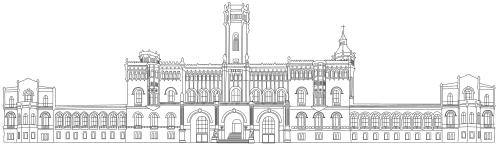
\includegraphics[height=4cm]{welfenschloss_vektor}
   \end{figure}

\vspace{1cm}

    {\LARGE \textsc{Leibniz Universität Hannover}}\\[1.0cm]

    {\Large \textsc{Institut für Antriebssysteme}} \\[0.2cm]
    {\Large \textsc{und Leistungselektronik}} \\ [0.4cm]

    {\Large \textsc{Fachgebiet Elektrische Maschinen}} \\ [0.2cm]
		{\Large \textsc{und Antriebssysteme}} \\ [1.7cm]

    {\Large \textbf{Titel \\[0.3cm] der Arbeit} } \\ [3cm]

    {\Large Diplomarbeit} \\ [1.5cm]

    {\large Vorname Name} \\
    {Matrikelnummer: xxxxxxx } \\ [1.5cm]

    \begin{tabular}{rl}
      Betreuer:    & Name Vorname\\
      Erstprüfer:  & Prof. Dr.-Ing. Bernd Ponick\\
      Zweitprüfer: & Prof. Dr.-Ing. Axel Mertens
    \end{tabular}

\end{center}

\end{titlepage}

% \clearpage{\thispagestyle{empty}\cleardoublepage}       %leere Seite für "documentclass book"

\chapter*{Eigenständigkeitserklärung}
\thispagestyle{empty}
\vspace{1cm}

\begin{flushleft}

Vorname Name \\
Straße Nr. \\
xxxxx Stadt

\vspace{1.0cm}

\begin{tabular}{@{} l l}
Matrikelnummer:  & xxxxxxx \\
Studienrichtung: & Energietechnik \\
\end{tabular}

\vspace{3.0cm}

Ich erkläre hiermit, dass ich die vorliegende Arbeit selbstständig
angefertigt und keine anderen als die angegebenen Quellen und
Hilfsmittel verwendet habe. \\ [2cm]

Hannover, den \today

\end{flushleft}

% \clearpage{\thispagestyle{empty}\cleardoublepage}       %leere Seite für "documentclass book"

% \chapter*{Aufgabenstellung}
\thispagestyle{empty}


Hier steht die Aufgabenstellung.

% \clearpage{\thispagestyle{empty}\cleardoublepage}       %leere Seite für "documentclass book"


%%%%%%%%%%%%%%%%%%%%%%%%%%%%%%%%%%%%%%%%%%%%%%%%%%%%%%%%%%%%%%%%%%%%%%%%%%%%%%%%%%%%%i1i1%%%%
%Inhaltsverzeichnis

\pagenumbering{roman}                               % Seitennummerierung arabische Zahlen
\tableofcontents
\clearpage      %leere Seite für "documentclass book"

%%%%%%%%%%%%%%%%%%%%%%%%%%%%%%%%%%%%%%%%%%%%%%%%%%%%%%%%%%%%%%%%%%%%%%%%%%%%%%%%%%%%%%%%%
%Abbildungsverzeichnis

\listoffigures
% \addcontentsline{toc}{chapter}{Abbildungsverzeichnis}   %Eintrag im InhaltsverzeichnisB
\addcontentsline{toc}{chapter}{List of figures}
\clearpage


%%%%%%%%%%%%%%%%%%%%%%%%%%%%%%%%%%%%%%%%%%%%%%%%%%%%%%%%%%%%%%%%%%%%%%%%%%%%%%%%%%%%%%%%%
%Tabellenverzeichnis

\listoftables
% \addcontentsline{toc}{chapter}{Tabellenverzeichnis}     %Eintrag im Inhaltsverzeichnis
\addcontentsline{toc}{chapter}{List of tables}   
\clearpage

\markboth{List of Symbols}{}                    %Kopfzeilenbeschriftung
\chapter*{List of Symbols}
\addcontentsline{toc}{chapter}{List of Symbols} %Eintrag im Inhaltsverzeichnis
\begin{tabular}{ll}
 
    $A$
        & Ampere\\
    $C$
        & Cycle\\
    $H$
         & Height\\
    $I$
         & Current\\
    $mAh$
        & Milliampere hour\\
    $mA$
        & Milliampere\\
    $mil$
        & Thousandth of an inch\\  
    $ms$
        & Millisecond\\
    $mV$
        & Millivolt\\
    $R$
        & Resistance\\

    $T$ & Time \\

    $U$
        & Voltage\\ 
    $V$
        & Volt\\
    $W$
        & Watt\\
    $\mu s$
        & Millisecond\\
    $\omega$
        & Ohm\\
    $\phi$ 
        &Sample command\\
\end{tabular}

%%%%%%%%%%%%%%%%%%%%%%%%%%%%%%%%%%%%%%%%%%%%%%%%%%%%%%%%%%%%%%%%%%%%%%%%%%%%%%%%%%%%%%%%%
% % Formelzeichenkonvention
% \markboth{List of Symbols}{}                    %Kopfzeilenbeschriftung
% \include{List of Symbols}
% % \markboth{Formelzeichenkonvention}{}    
% % \chapter*{List of Symbols}
\addcontentsline{toc}{chapter}{List of Symbols} %Eintrag im Inhaltsverzeichnis
\begin{tabular}{ll}
 
    $A$
        & Ampere\\
    $C$
        & Cycle\\
    $H$
         & Height\\
    $I$
         & Current\\
    $mAh$
        & Milliampere hour\\
    $mA$
        & Milliampere\\
    $mil$
        & Thousandth of an inch\\  
    $ms$
        & Millisecond\\
    $mV$
        & Millivolt\\
    $R$
        & Resistance\\

    $T$ & Time \\

    $U$
        & Voltage\\ 
    $V$
        & Volt\\
    $W$
        & Watt\\
    $\mu s$
        & Millisecond\\
    $\omega$
        & Ohm\\
    $\phi$ 
        &Sample command\\
\end{tabular}


%%%%%%%%%%%%%%%%%%%%%%%%%%%%%%%%%%%%%%%%%%%%%%%%%%%%%%%%%%%%%%%%%%%%%%%%%%%%%%%%%%%%%%%%%
%Formelzeichenverzeichnis

% \markboth{Formelzeichenverzeichnis}{}                    %Kopfzeilenbeschriftung
% %Präfix [] Konvention

%Lateinische Buchstaben bekommen im Präfix ein A
%Griechische Buchstaben bekommen im Präfix ein G
%Hochgestellte Indizes bekommen im Präfix ein X
%Indizes bekommen im Präfix ein Z
%Großbuchstaben bekommen im Präfix ein g angehängt

%Griechische Zeichen: zweistellige Nummerierung nach Stellung im Alphabet
    %alpha-01   beta-02     gamma-03    delta-04     epsilon-05   zeta-06     eta-07        theta-08
    %iota-09    kappa-10    lambda-11   mu-12        nu-13        xi-14       omicron-15    pi-16
    %rho-17     sigma-18    tau-19      upsilon-20   phi-21       chi-22      psi-23        omega-24
%Lateinische Zeichen: Lateinisches Zeichen

%\nomenclature[]{$$}{}{}{}

%%%%%%%%%%%%%%%%%%%%%%%%%%%%%%%%%%%%%%%%%%%%%%%%%%%%%%%%%%%%%%%%%%%%%%%%%%%%%%%%


\nomenclature[G03]{$\gamma$}{Kleines Gamma}{$\SI{}{\newton\meter}$}{}

\nomenclature[G03g]{$\Gamma$}{Großes Gamma}{$\SI{}{\meter\per\second}$}{}

\nomenclature[ABg]{$B$}{Großes B}{$\SI{}{\meter\per\second}$}{}

\nomenclature[Ab]{$b$}{Kleines B}{}{}

\nomenclature[ZUg]{$U$}{Großes U}{}{}

\nomenclature[Zu]{$u$}{Kleines u}{}{}

\nomenclature[XFg]{$F$}{Großes F}{}{}

\nomenclature[Xf]{$f$}{Kleines f}{}{}

% \printnomenclature                                       %Verzeichnis drucken
% \clearpage{\pagestyle{empty}\cleardoublepage}            %leere Seite für "documentclass book"


%%%%%%%%%%%%%%%%%%%%%%%%%%%%%%%%%%%%%%%%%%%%%%%%%%%%%%%%%%%%%%%%%%%%%%%%%%%%%%%%%%%%%%%%%
%Kapitel & Anhang

%%%%%%%%%%%%%%%%%%%%%%%%%%%%%%%%%%%%%%%%%%%%%%%%%%%%%%%%%%%%%%%%%%%%%%%%%%%%%%%%%%%%%%%%%
%Kapitel

\pagenumbering{arabic}                                  % Seitennummerierung arabische Zahlen
\chapter{Einleitung}
\label{chap:Einleitung}


Die vorliegende Arbeit11...1

\chapter{Fundamentals}
\label{chap:Fundamentals}
This chapter introduces the basic knowledge of the measurement system modules and the basic structure of the corresponding circuit, and introduces several applications related to the Internet, which can handle the measurement results well.The measured current value can be obtained by Ohm's law by measuring the voltage, so this article only collects the voltage value to measure the voltage value and the current value.
\section{ADC}
\label{sec:ADC}
% 2.1
In order to plan long-term measurement measurement devices, we must first understand the basic types of ADCs, the characteristics of each type, and their accuracy. In addition, you need to understand the basic circuit of the specific selection of the microcontroller, and you can know how the ADC performs voltage measurement.

\subsection{Introduction of voltage/current-sensor}
\label{sec:Introduction of voltage/current-sensor}
%2.1.1


The essence of voltage/current-sensor sensor measuring voltage is a voltage divider circuit composed of resistors. Its principle is the knowledge of resistor series voltage divider. The typical circuit is shown in Figure ~\ref{fig:2.1}. 
\begin{figure}[h]
	\centering
% [width=13cm]         [scale=0.9]
	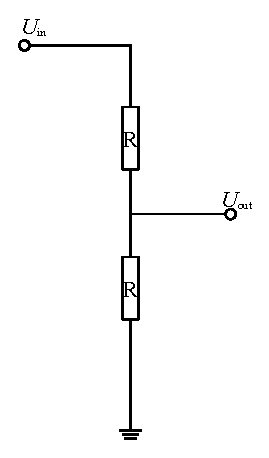
\includegraphics{grafiken/2.1.eps}
	\caption{Structure of divider resistor} 
	\label{fig:2.1}
\end{figure}
Here, $\cdot U_{in}$ is the voltage of component under test, $\cdot U_{out}$ is voltage of divider resistor R2, and $\cdot R_{1}$, $\cdot R_{2}$ are divider resistors.
\\
Therefore, the measured voltage provided to the ADC channel is the following formula:
\\
\begin{center} 
\begin{equation}
 U_{out} = \frac{R_{2}}{R_{1}+R_{2}} U_{in}  
\end{equation}
\end{center}

There are a variety of precision ADCs available on the market to choose from, as shown in the Figure~\ref{fig:2.2} below , the appropriate ADC precision can be selected according to the signal bandwidth, so that it is convenient for users to measure.
\begin{figure}[h]
	\centering
	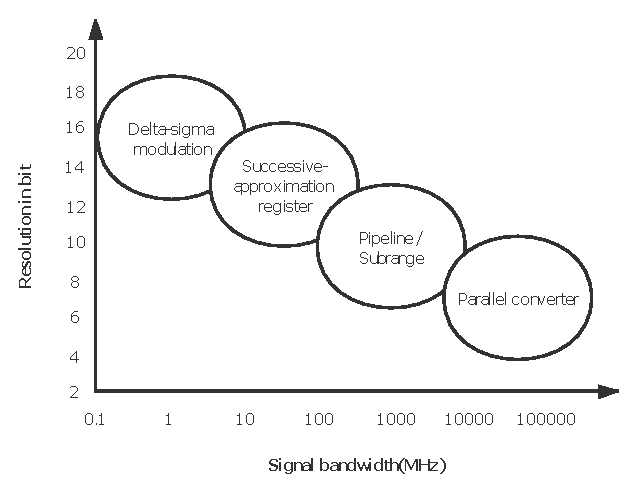
\includegraphics{grafiken/2.2.eps}
	\caption{ADC-Architecture depending on signal bandwidth and resolution} 
	\label{fig:2.2}
\end{figure}
\\
In the case of methods without feedback, the parallel converter has the simplest structure, which is why, with high resolution, a large number of components with high demands on accuracy are required. Here, too, there are methods with range selectivity, oversampling and ramp methods. A folding process has also established itself alongside a multiplex technique. 
\\
The following Figure~\ref{fig:2.3} briefly describes the basic structure of the parallel converter:
\begin{figure}[h]
	\centering
	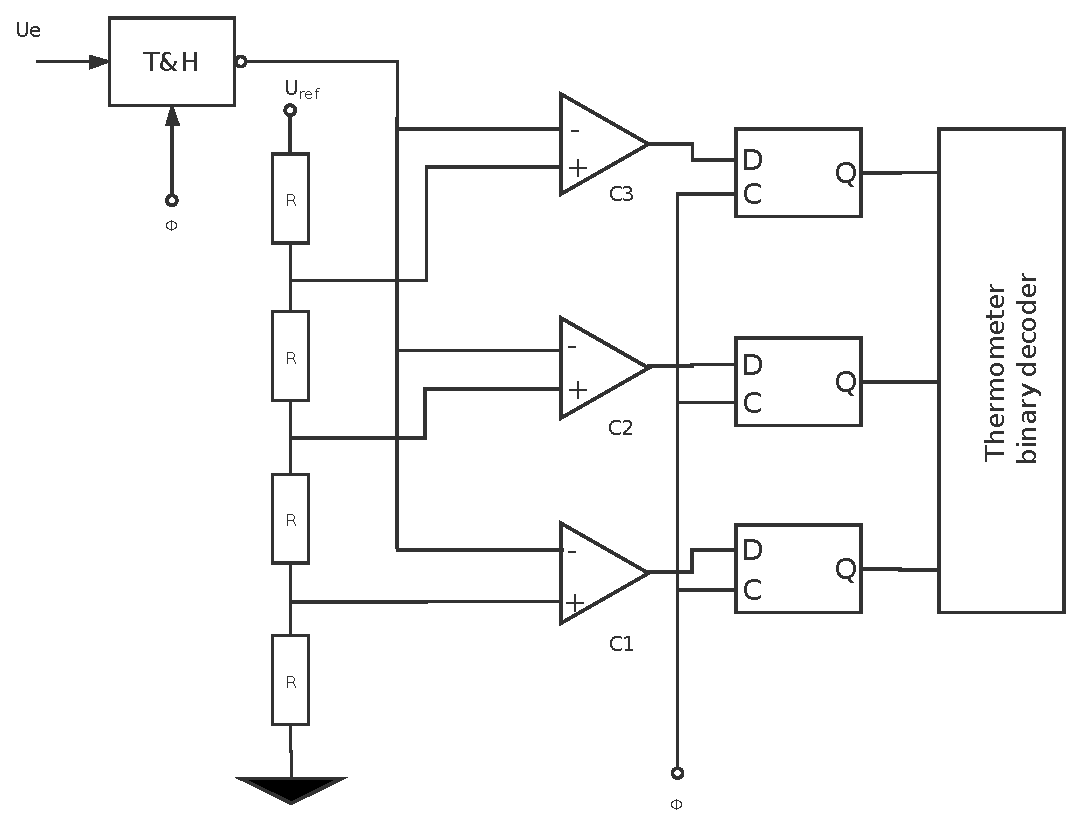
\includegraphics[width=15cm]{grafiken/2.3.eps}
	\caption{Block diagram of a parallel converter} 
	\label{fig:2.3}
\end{figure}
\\
Since with this parallel converter (flash converter) the entire conversion takes place within one clock period, it is the fastest method. It is easy to see, however, that the number of components required quickly becomes very large, since the entire chain with resistor, comparator and latch is required for each of the $2^{n}-1$ comparison values. The thermometer code present at the output of the latches is encoded in a binary code (often a Gray code, in which neighboring numbers differ by only one bit). Differential amplifiers are particularly suitable as comparators, with the gain v having to be at least so large that $\Delta U/2$ is sufficient to control the necessary logic level of the latches.
\\
The second important method is called the weighing method, which requires feedback via a digital-to-analog converter, as Figure ~\ref{fig:2.4} shows.
\begin{figure}[h]
	\centering
	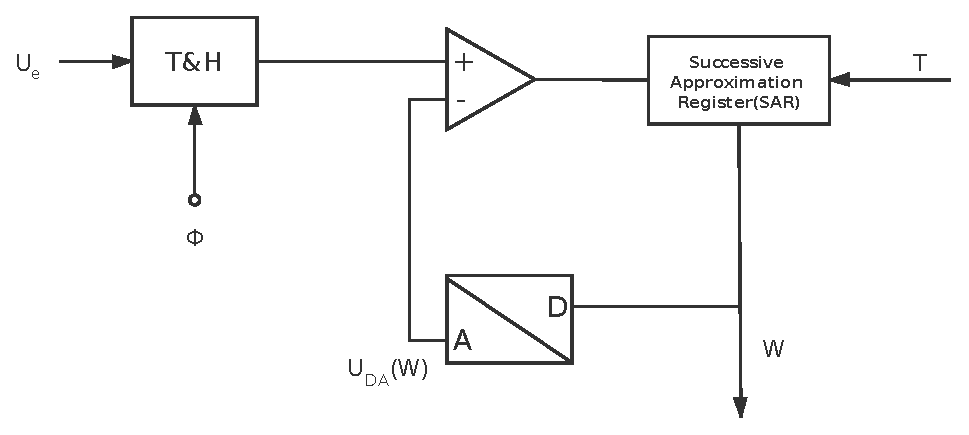
\includegraphics{grafiken/2.4.eps}
	\caption{Converter according to the weighing method} 
	\label{fig:2.4}
\end{figure}
 As soon as the track and hold element (T\&H) has switched to hold mode, the weighing cycle begins with the most significant bit. If $ u_{e}>\frac{U_{max}}{2} $, the top bit remains set and the second bit is set to 1 on a trial basis.
\\
The comparator decides whether the word in the SAR is smaller than the input signal. Then the check bit remains set and the next lowest bit is checked. If  $u_{e}<u_{DA}(W)$, the check bit is reset.
\\
The conversion time is n clock periods, whereby the digital-to-analog converter must have full accuracy. The advantage of high resolutions is that only one precise comparator is required. This enables the design of very energy efficient implementations.
If a counter is used instead of the SAR, the Laund can count the clock cycles backwards through the comparator. In the steady state, the data word indicates. There are also many variants of this counting method, whereby in the worst case the conversion time can be up to $2^{n}$ clock cycles.
In the gallium nitride measurement, because the precision is required but the precision is not the highest, the above-mentioned method is selected.

\subsection{ADC in microcontroller STM32F303ZET}
\label{sec:ADC in microcontroller STM32F303ZET}
% 2.1.2
In this measurement, we choose STM32F303ZET as a microcontroller containing multiple 12-bit precision ADCs. Its core is ARM-Cortex-M4, and its ADC is of type Successive approximation register.
Each stm32F303 has a 40-channel independent 16-bit precision ADC, and the price is very high, so we choose this microcontroller to measure the voltage signal to determine whether the gallium nitride is affected by cosmic rays. The following Figure~\ref{fig:2.5} is the typical connection diagram using the ADC:
\begin{figure}[h]
	\centering
	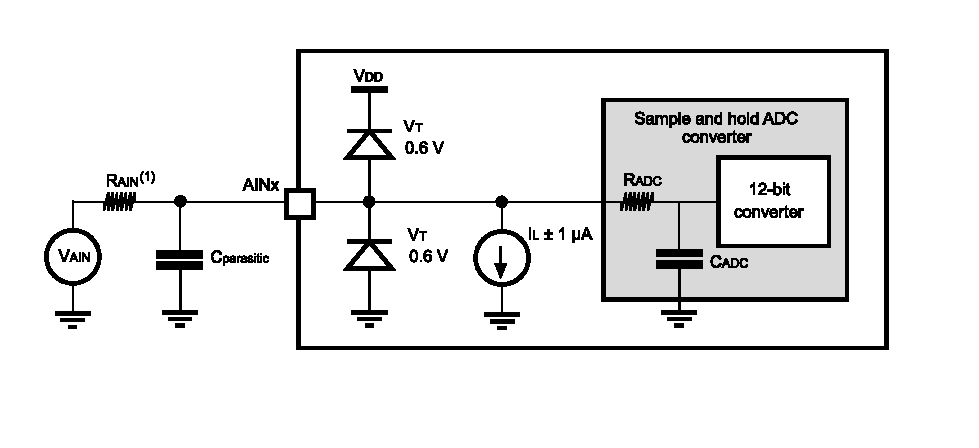
\includegraphics{grafiken/2.5.eps}
	% datasheet 144/173
	\caption{Typical connection diagram using the ADC} 
	\label{fig:2.5}
\end{figure}
\section{Ethernet}
\label{sec:Ethernet}
% 2.2
Ethernet has very extensive and in-depth applications in various fields and industries. This is mainly due to the high flexibility and ease of implementation of Ethernet. Because Ethernet has the advantages of simple networking, low cost, excellent compatibility, reliable connection, and convenient topology adjustment, it has advantages that other network technologies do not have in terms of being a gateway for smart homes, Internet of Things or wireless sensor networks. , Thus get vigorous development and application. This article will introduce in detail how to connect the embedded system to the Ethernet, how to use the hardware protocol stack to make your solution or application connect to the Internet quickly and efficiently, how to realize TCP/IP communication, and how to realize the upper application layer protocol and many more.
\subsection{Introduce of W5500}
\label{sec:Introduce of W5500}
% 2.2.1
The W5500 network expansion board integrates a hardware TCP/IP protocol stack chip W5500 and an RJ-45 with a network transformer. Among them, W5500 is a full hardware TCP/IP embedded Ethernet controller, which provides a simpler Internet connection solution for embedded systems. Hardware logic gate circuits are used to implement the transmission layer and network layer of the TCP/IP protocol stack (such as : TCP, UDP, ICMP, IPv4, ARP, IGMP, PPPoE and other protocols), and integrates the data link layer, physical layer, and 32K bytes of on-chip RAM as a data receiving and sending buffer. Make the host computer main control chip only need to undertake the processing task of TCP/IP application layer control information. This greatly saves the workload of the host computer for data replication, protocol processing, and interrupt processing, and improves system utilization and reliability. 
\\
Its module structure is shown in the Figure~\ref{fig:2.6} below:
\\
\begin{figure}[h]
	\centering
	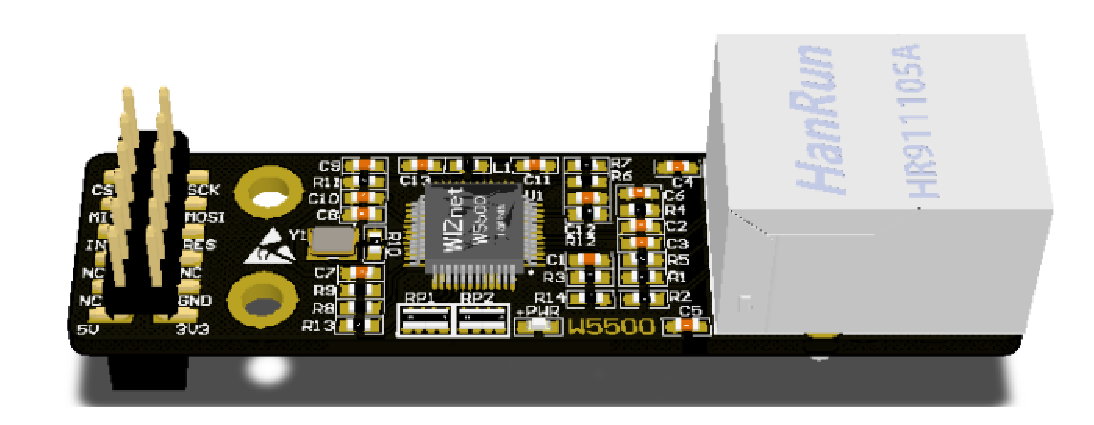
\includegraphics[width=15cm] {grafiken/2.6.eps}
	\caption{Physical model of W5500} 
	\label{fig:2.6}
\end{figure}
W5500 supports 8 sockets at the same time to facilitate communication with different IPs and devices; in order to reduce system energy. W5500 provides Wake-on-LAN mode (WOL) and power-down mode for customers to choose to use; W5500 is non-aggressive. The hardware network engine can prevent similar torrent, fraud and injection network attacks and improve network security.

\subsection{solution of ethernet access}
\label{sec:solution of ethernet access}
% 2.2.2
For non-operating system, how does the single-chip microcomputer required by the system realize network access? I will categorize these schemes according to the different TCP/IP protocol stacks below.
\\
It is divided into two categories: the first category is the traditional software TCP/IP protocol stack solution; the second category is the latest hardware TCP/IP
Protocol stack scheme. Below I will analyze the implementation of these two types of solutions: 
\\
1) MAC+PHY solutions:

\begin{figure}[!ht]
	\centering
	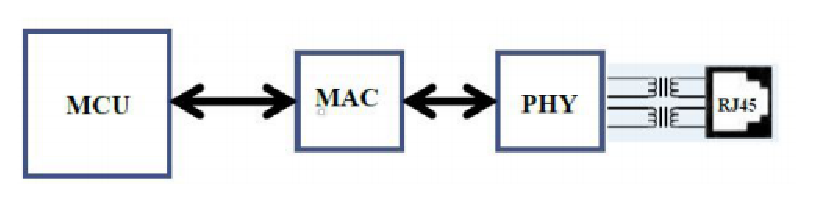
\includegraphics[width=15cm] {grafiken/2.7.eps}
	\caption{MAC+PHY Ethernet solution} 
	\label{fig:2.7}
\end{figure}
\FloatBarrier
The traditional Ethernet access scheme is as shown in the figure below. The MCU+MAC+PHY is added to the network interface to realize the Ethernet
The physical connection of the network realizes communication and upper-layer applications by implanting TCP/IP protocol code in the main control chip.
\\
2) Hardware protocol stack chip solution: 
\begin{figure}[!ht]
	\centering
	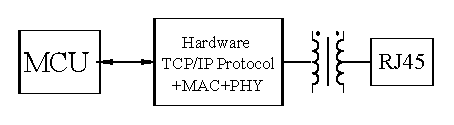
\includegraphics[width=15cm]{grafiken/2.8.eps}
	\caption{Hardware protocol stack chip solution} 
	\label{fig:2.8}
\end{figure}
\FloatBarrier
The hardware protocol stack chip scheme is shown in the figure below. The MCU + hardware protocol stack chip (including MAC and PHY) directly adds the network interface, and the single-chip microcomputer can be easily connected to the network. All the work of processing the TCP/IP protocol is through the "little secretary" of the MCU-the hardware protocol Stack chips to complete.
\\
This solution was first proposed by WIZnet and successfully launched the Ethernet series of chips: W5100, W5200, W5300 and W5500. The so-called hardware protocol stack refers to the implementation of the traditional software TCP/IP protocol stack with hardware-based logic gate circuits, as shown in the Figure~\ref{fig:2.9} below.
\begin{figure}[!ht]
	\centering
	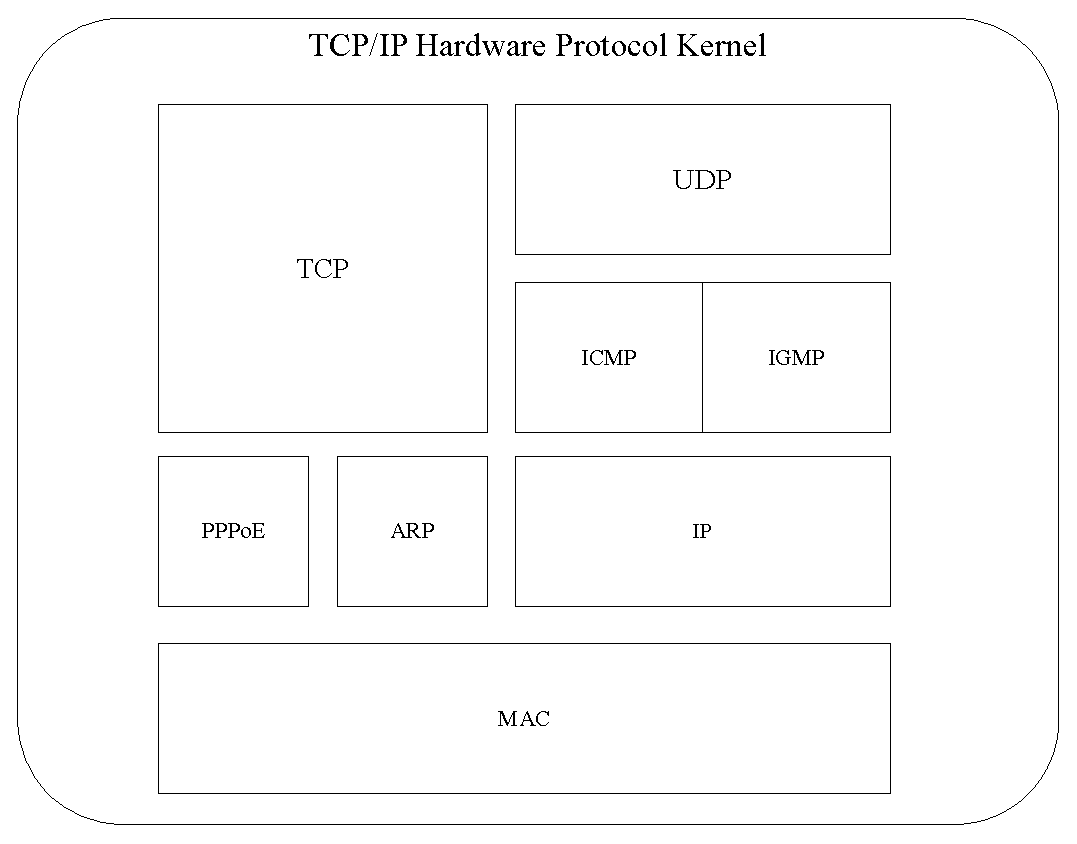
\includegraphics[scale=0.85]{grafiken/2.9.eps}
	\caption{Hardware protocol kernel} 
	\label{fig:2.9}
\end{figure}
\FloatBarrier
The core of the Ethernet chip is composed of protocols such as TCP, UDP, ICMP, IGMP in the transport layer, IP, ARP, PPPoE and other protocols in the network layer, and MAC in the link layer, plus physical layer PHY and peripheral registers and memory The SPI interface constitutes this complete set of hardware-based Ethernet solutions.
\\
This hardware TCP/IP protocol stack replaces the previous MCU to handle these interrupt requests. That is, the MCU only needs to process user-oriented application layer data. The transmission layer, network layer, link layer and physical layer are all controlled by the peripheral WIZnet The chip is complete. This set of solutions simplifies the aforementioned five-layer network model from two aspects of hardware overhead and software development, and simplifies product development solutions. In this way, engineers no longer have to face the cumbersome communication protocol code, only need to understand the simple register function and Socket programming to complete the network function development part of the product development work.

\section{SMTP}
\label{sec:SMTP}
% 2.10
When collecting temperature signals, if the state of more than 50 units under test suddenly changes within 10s, it is likely to be a manual error. At this time, it is necessary to set up an email-related program in the measurement system to send an email to notify the researcher. This article uses the SMTP protocol.
SMTP stands for Simple Mail Transfer Protocol. It is a group of mails used to transfer mail from source address to destination address
Rules, which control the way in which letters are transferred. The actual process of sending emails can be shown in Figure~\ref{fig:2.10}:
 
% ~\ref{fig:2.10} 
\begin{figure}[!ht]
	\centering
	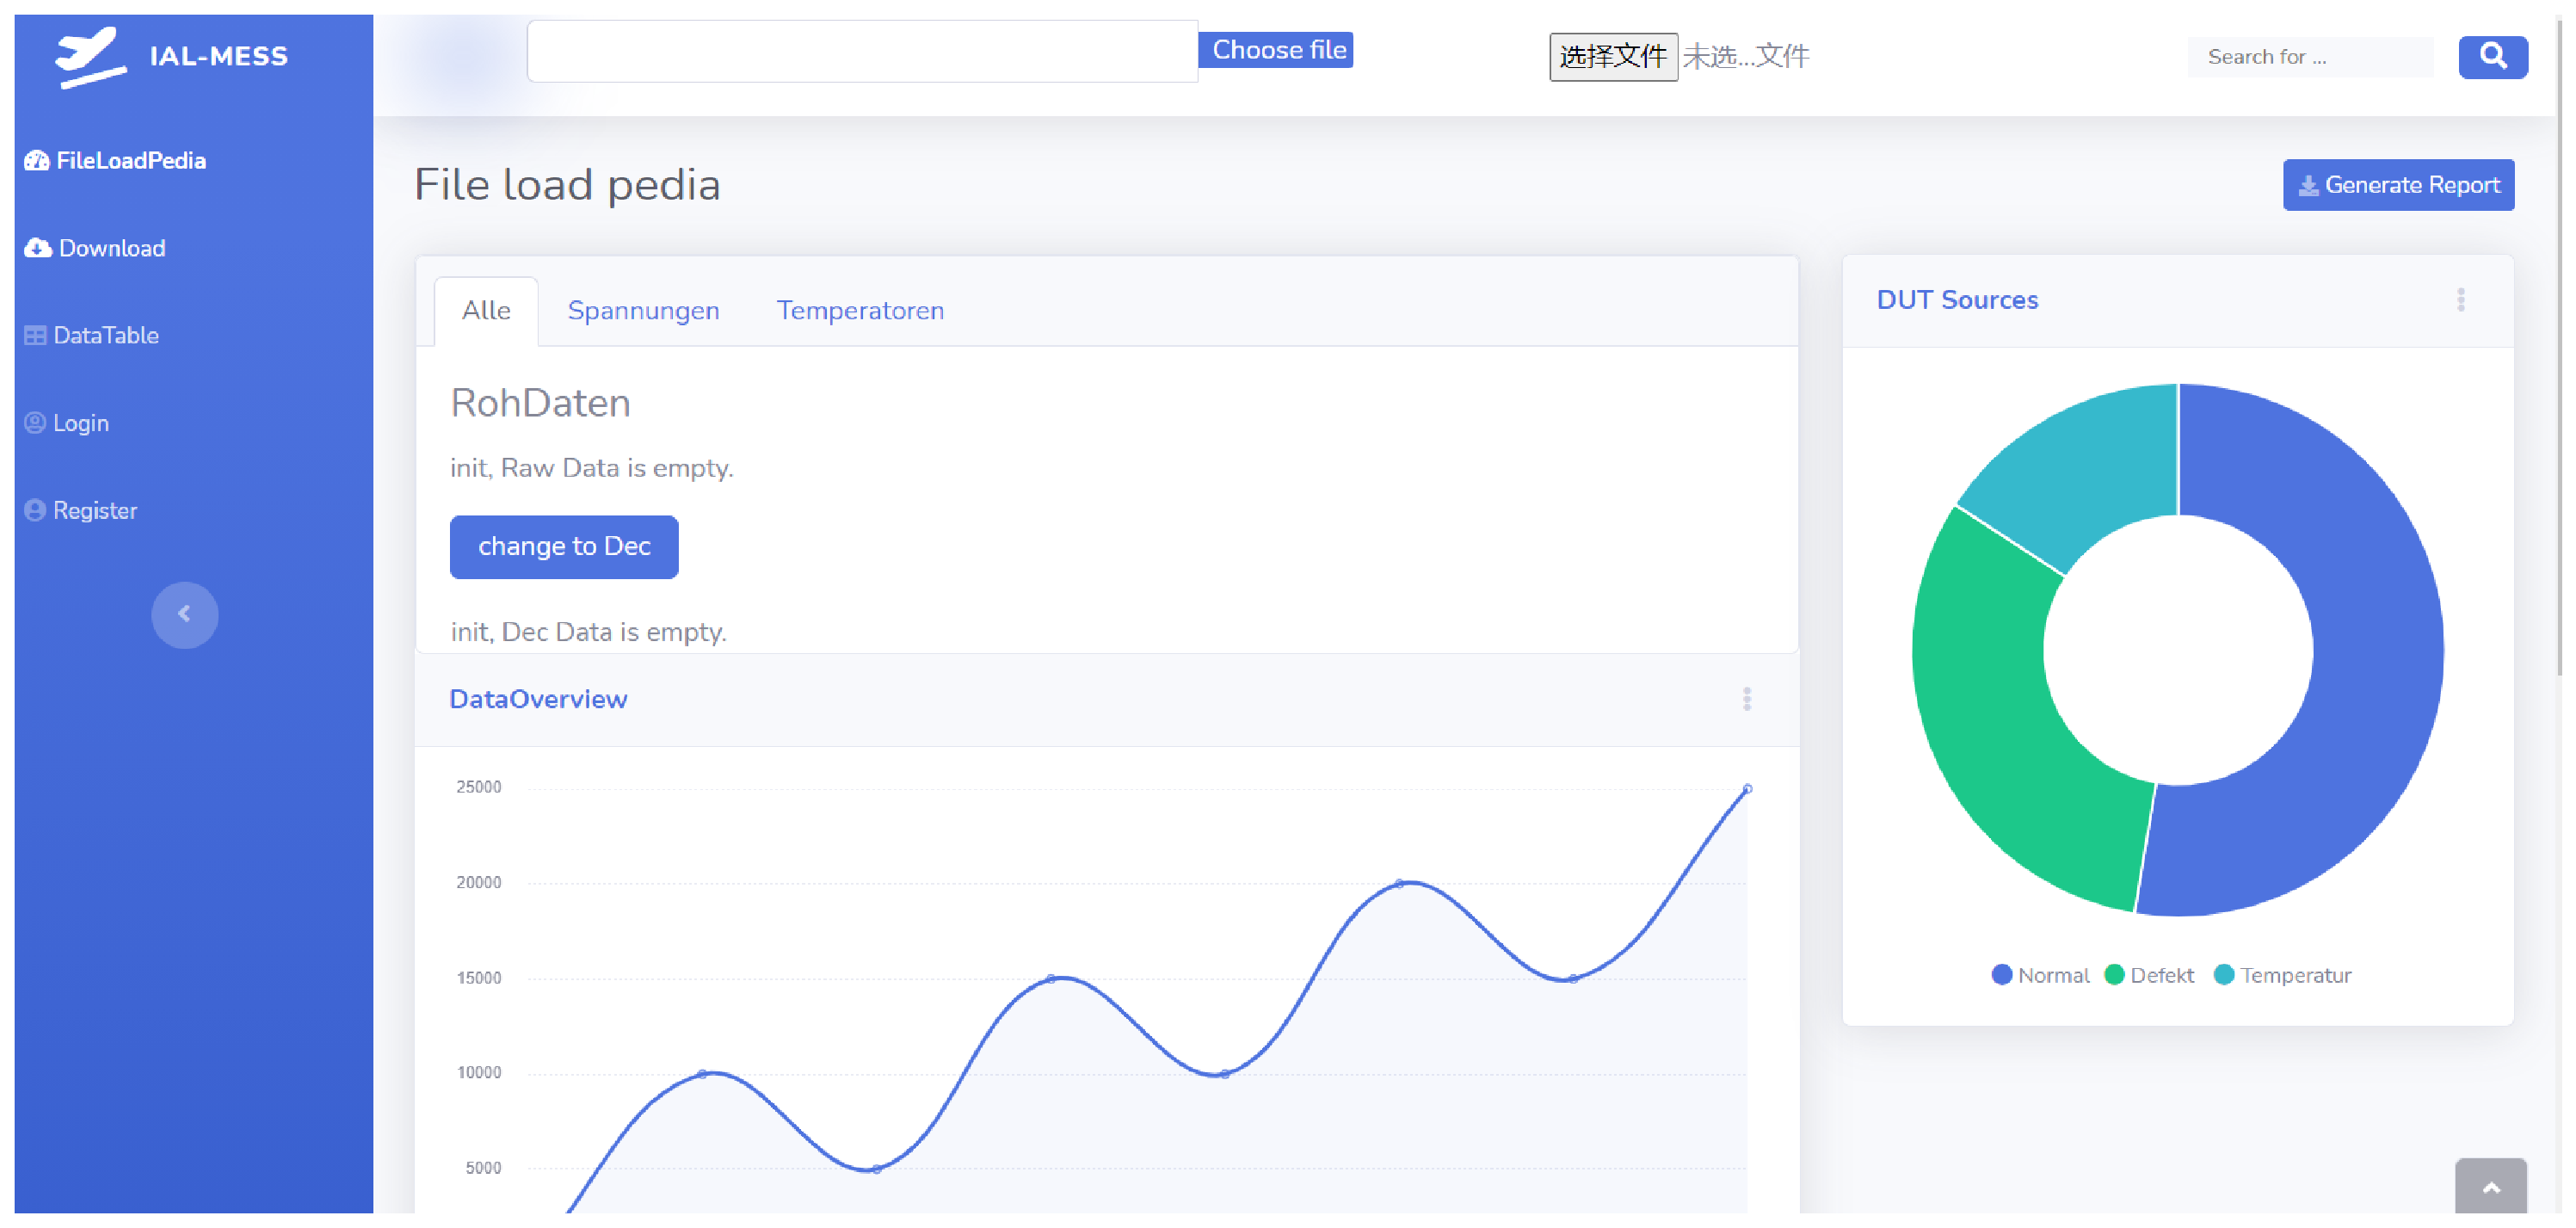
\includegraphics[width=15cm]{grafiken/2.10.eps}
	\caption{Schematic diagram of the mail sending process} 
	\label{fig:2.10}
\end{figure}
\FloatBarrier

An important feature of it is that it can relay mail during transmission, that is, mail can be relayed through hosts on different networks. Usually it works in two situations: one is the transmission of mail from the client to the server; the other is the transmission from one server to another server. SMTP is a request/response protocol, it monitors port 25, is used to receive the user's Mail request, and establish an SMTP connection with the remote Mail server.
\\
SMTP usually has two working modes. Send SMTP and receive SMTP. The specific working method is: Send SMTP after receiving the user's mail request, determine whether the mail is a local mail, if it is directly delivered to the user's mailbox, otherwise query the MX record of the remote mail server to the DNS, and establish a connection with the remote A two-way transmission channel between receiving SMTP, after which SMTP commands are issued by the sending SMTP, received by the receiving SMTP, and the response is transmitted in the opposite direction. Once the transmission channel is established, the SMTP sender sends a MAIL command to indicate the sender of the mail. If the SMTP receiver can receive the mail, an OK response is returned. The SMTP sender then issues the RCPT command to confirm whether the mail has been received. If the SMTP receiver receives it, it will return an OK response; if it cannot receive it, it will send a rejection response (but not stop the entire mail operation), and both parties will repeat this many times. When the receiver receives all the mails, it will receive a special sequence. If the receiver successfully processes the mail, it will return an OK response.
\\


\section{UDP}
\label{sec:UDP}
% 2.4
In the transport layer of the TCP/IP protocol stack, TCP is connection-oriented, and the UDP protocol to be demonstrated next. It is non-connection oriented.
\\
When UDP transmitting data, there is no confirmation, retransmission, or congestion mechanism. Since this measurement can obtain a large amount of data in a short time, the packet loss and error data can be verified by the large amount of data received later, so this time we choose UDP.
\\
Compared with TCP, UDP does not return a response signal for each received frame during transmission. When network transmission fails, such as a router restart and the network is suddenly interrupted, UDP can still receive the signal transmitted by the server as much as possible. The comparison figure~\ref{fig:2.11}  is as follows :
% ~\ref{fig:2.11} 
\begin{figure}[!ht]
	\centering
	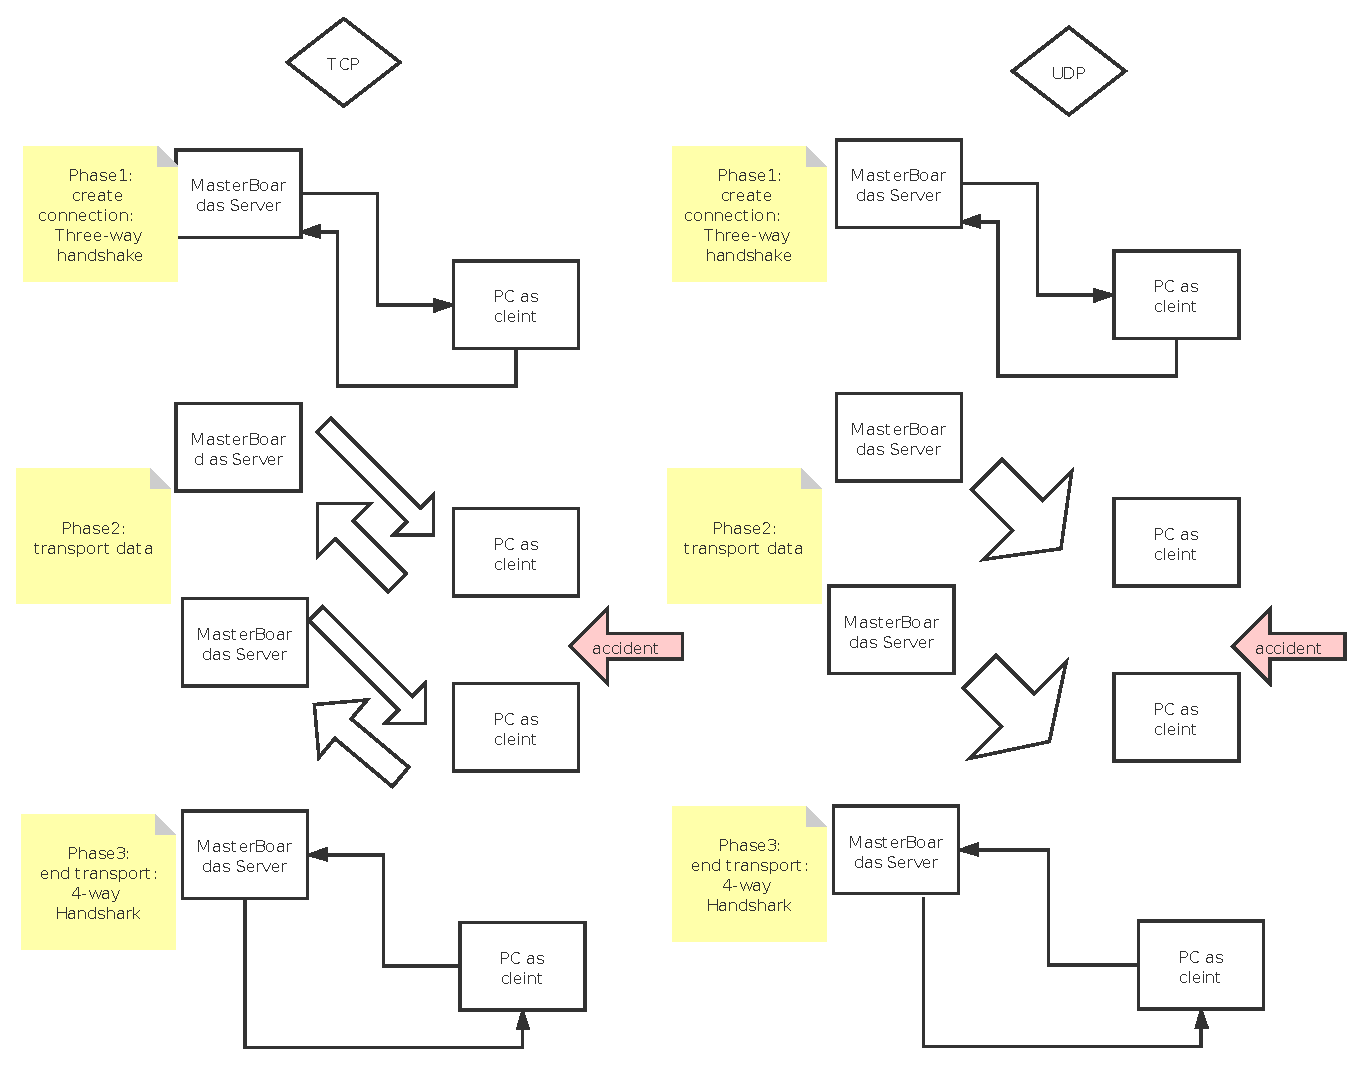
\includegraphics[scale=0.7]{grafiken/2.11.eps}
	\caption{Comparison of TCP and UDP} 
	\label{fig:2.11}
\end{figure}
\FloatBarrier
The UDP establishment process of W5500 is also very convenient, which can be easily realized by simply reading and writing registers. After the program is initialized, enter the main loop function. When the Socket is closed, before communicating, we first initialize the Socket port in UDP mode. When the socket is in the initialization completed state, that is, the SOCK UDP state, data can be sent by broadcast at this time.
\\
Next, use W5500 to demonstrate how to use UDP to send and receive data. There are two issues to pay attention to before the test. 
\\
First, it is recommended to turn off the PC firewall.
\\
Secondly, if the W5500 module and the PC are directly connected via a network cable, you need to modify the IP address of the PC to a static IP, and keep it in the same network segment as the W5500 IP. 
\\
If you connect to the router directly, you do not need to modify the IP address of the PC. The specific test steps are:
\\
1. Use the IP address obtained by the router to set the configuration file in the W5500, this IP must be in the same network segment as the router gateway.
\\
2. Obtain the computer IP address through the command line and write it as remote IP into the configuration file of the w5500 Ethernet chip.
\\
3. Compile the code, and then burn the program to the Wildfire development board.
\\
4. Connect the network cable and USB serial port cable. Open the serial port debugging tool, reset the Wildfire development board, and get the setting information from the output result.

\section{SPI}
\label{sec:SPI}
% 2.5
The Serial Peripheral Interface (SPI) is a synchronous serial communication interface specification used for short-distance communication, primarily in embedded systems. The interface was developed by Motorola in the mid-1980s and has become a de facto standard. Typical applications include Secure Digital cards and liquid crystal displays.
\\
SPI devices communicate in full duplex mode using a master-slave architecture with a single master. The master device originates the frame for reading and writing. Multiple slave-devices are supported through selection with individual slave select (SS), sometimes called chip select (CS), lines.
\\
Sometimes SPI is called a four-wire serial bus, contrasting with three-, two-, and one-wire serial buses. The SPI may be accurately described as a synchronous serial interface,[1] but it is different from the Synchronous Serial Interface (SSI) protocol, which is also a four-wire synchronous serial communication protocol. The SSI protocol employs differential signaling and provides only a single simplex communication channel. SPI is one master and multi slave communication.
\\
The figure~\ref{fig:2.12}  below is a standard SPI transmission process:
% ~\ref{fig:2.11} 
\begin{figure}[!ht]
	\centering
	
\includegraphics[width=15cm]{grafiken/2.12.pdf}
	\caption{standard SPI transmission process} 
	\label{fig:2.12}
\end{figure}
\FloatBarrier

\section{DMA}
\label{sec:DMA}
% 2.6
The basic definition of DMA: 
DMA has the full name of Direct Memory Access 
DMA transmission copies data from one address space to another address space, so as to realize high-speed data transmission between peripherals and memories or between memories. When CPU initializes such a transmission action, the transmission action is realized and completed through the DMA controller. The DMA transmission mode is dispense with CPU to realize direct control transmission or differing from the interrupt processing mode, it will reserve the site and recover the site process. Through RAM and IO devices, a channel of direct transmission data can be opened to improve CPU efficiency strongly. 

Main features of DMA:
Each channel is directly connected with the exclusive hardware DMA request. Each channel also supports software touch. Such functions can be configured through software; 
On the same DMA module, the priority between multiple requests can be established through software programming (with a total of four levels: very high, high, medium, and low). When the priority setting is equal, it depends on hardware (request 0 precedes over request 1, and the rest may be deduced by analogy); 
For the transmission width of independent data sources and target data areas (byte, half-word, and full-word), byte control is used in this design to simulate the process of packing and unpacking. The source and target address must be aligned according to the data transmission width; 
The buffer management can support circulation; 
Each channel has three event flags (DMA semi-transmission, DMA transmission completion, and DMA transmission error). The logic of three event flags may become an individual interrupt request; 
Transmission between memories, transmission between peripherals and memories, and transmission between memories and peripherals; 
Flash memory, SRAM, SRAM of peripherals, APB1, APB2, and AHB peripherals can be used as sources and targets for access; 
The maximum number of programmable data transmission is 65535. 
STM32F429 series chip DMA controller 
STM32F429 series chip at most has two DMA controller. DMA1 and DMA2 respectively includes 8 channels. Each channel specializes in managing the request of one or multiple peripheral for memory access. It also has the priority of coordinating each DMA request through arbitration. 

For the requests generated from peripherals (TIM, ADC, SPI1, SPI/I2S2, I2C and USART), it is inputted to DMA1/DMA2 controller through logic, implying that only one request is valid at the same time. 
DMA’s work block diagram is stated below: 
~\ref{fig:2.13}  of DMA:
% ~\ref{fig:2.12} 
\begin{figure}[!ht]
	\centering
	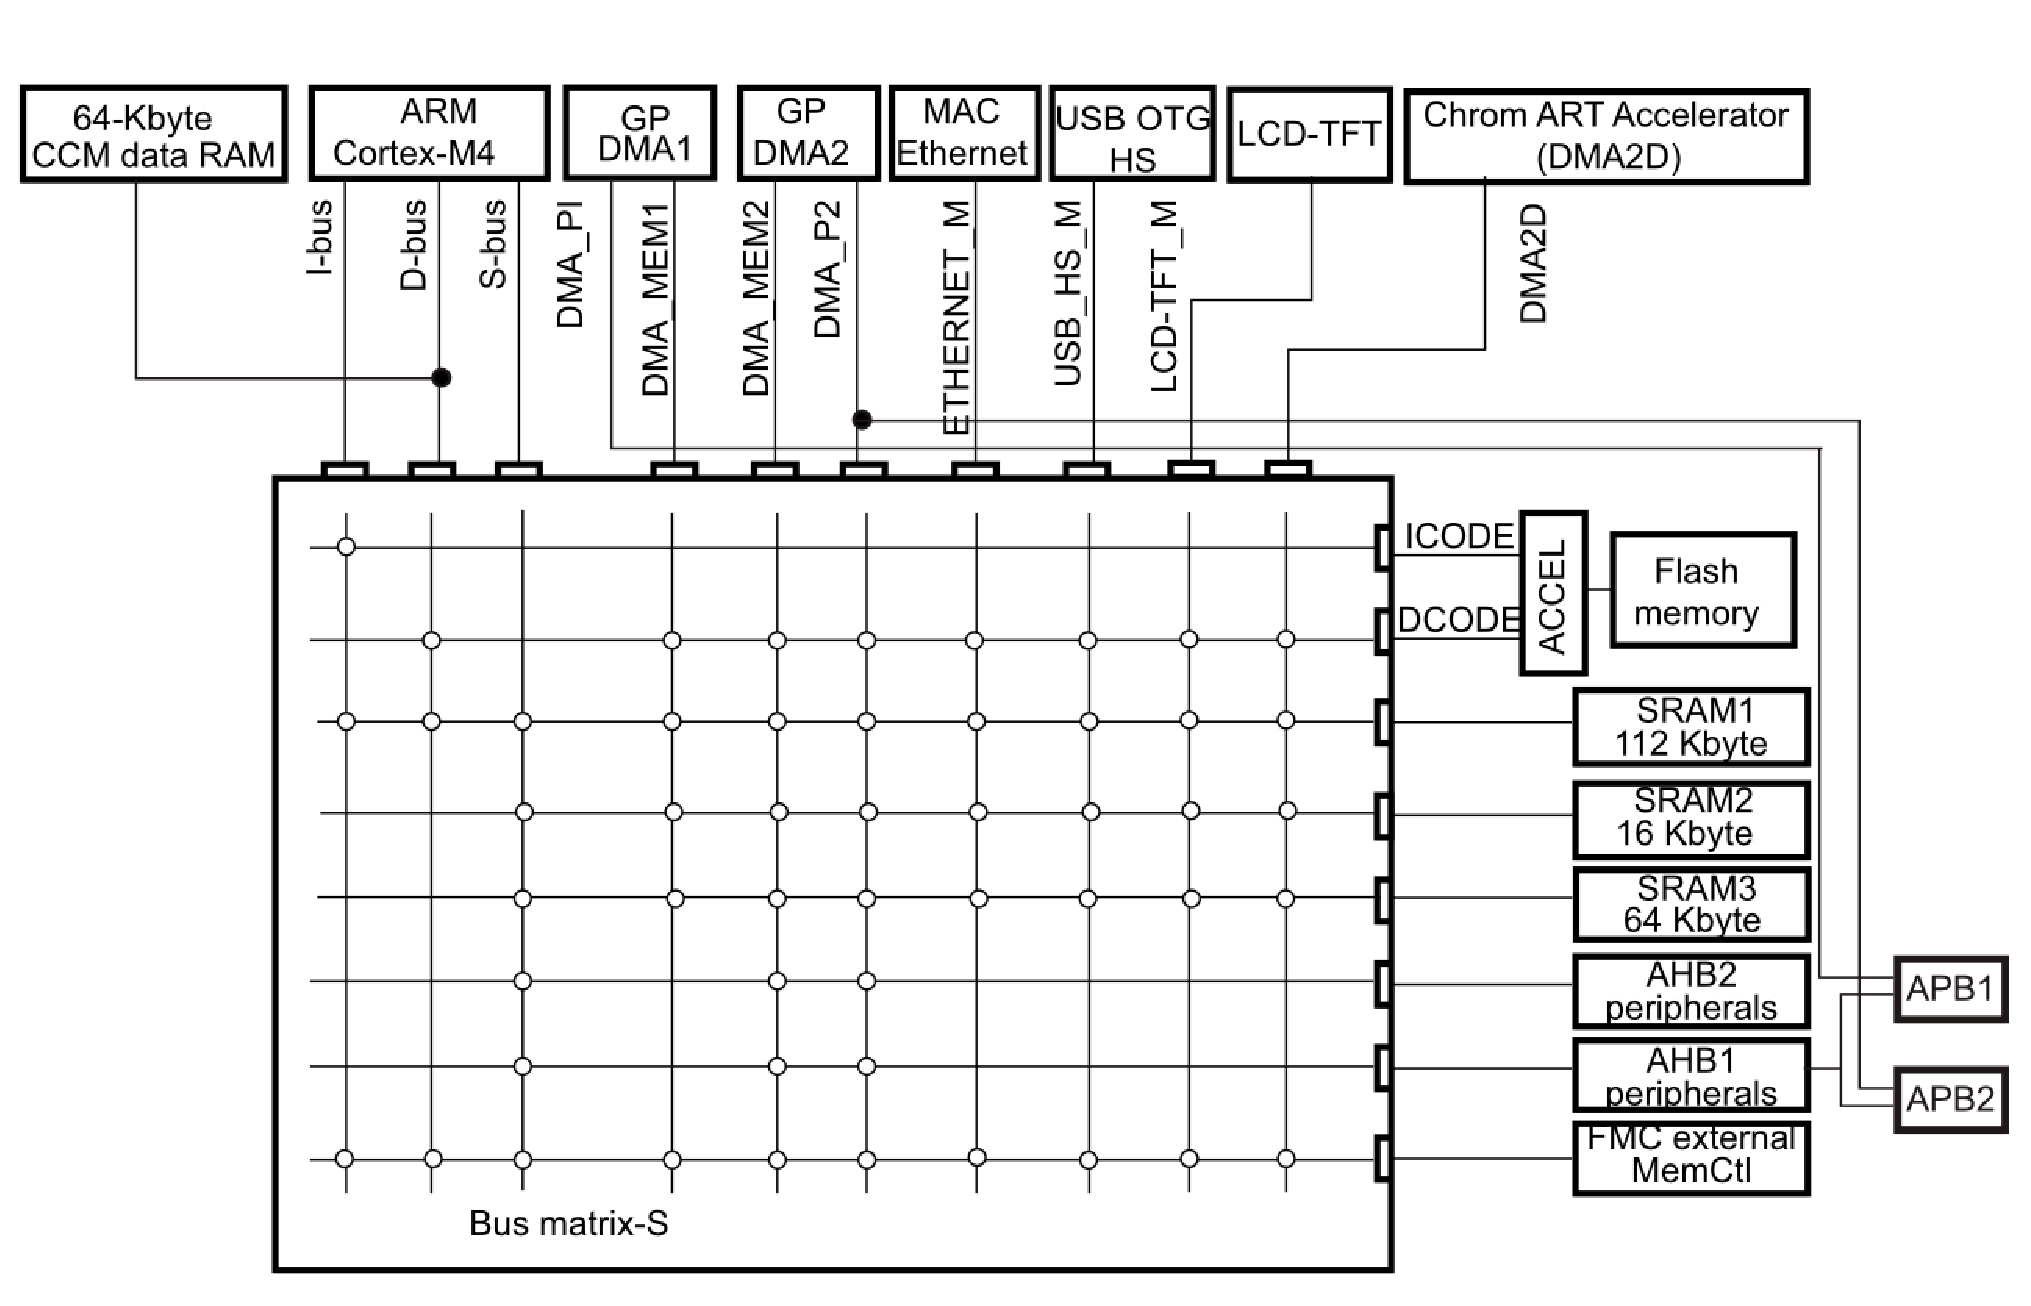
\includegraphics[width=15cm]{grafiken/2.13.eps}
	\caption{STM32F429xx Multi-AHB matrix} 
	\label{fig:2.13}
\end{figure}
\FloatBarrier

\section{Ngrok}
\label{sec:Ngrok}
% 2.7
Internal network penetration or NAT penetration aims to make the data package with a specific source IP address and source port number not block from NAT but will route to the internal network host correctly. The internal network penetration method is introduced through the relative position between the mutual communication host in the network and NAT devices. 
The UDP’s internal network penetration, in essence, uses the NAT system on the router. NAT is a conversion technology that transforms the private (reserved) address into the legal IP address. It is widely applied in the internet access ways with all kinds of types and different types of networks. NAT can reuse the address and realize external shelter for the internal network structure. 
Ngrok is a commonly used internal network penetration technology. Generally speaking, our local PC has two IPv4 addresses. One local IP is allocated by the router and the other one is the public network IP. However, people in other areas all over the world cannot directly use such two IP addresses to access the local PC. If the project’s logic and data structure are not complicated, developers can use the open-source ngrok for the internal network penetration so that external personnel can access the local PC. 
The following Figure~\ref{fig:2.14}  is a common application structure diagram of NAT.
% ~\ref{fig:2.14} 
\begin{figure}[!ht]
	\centering
	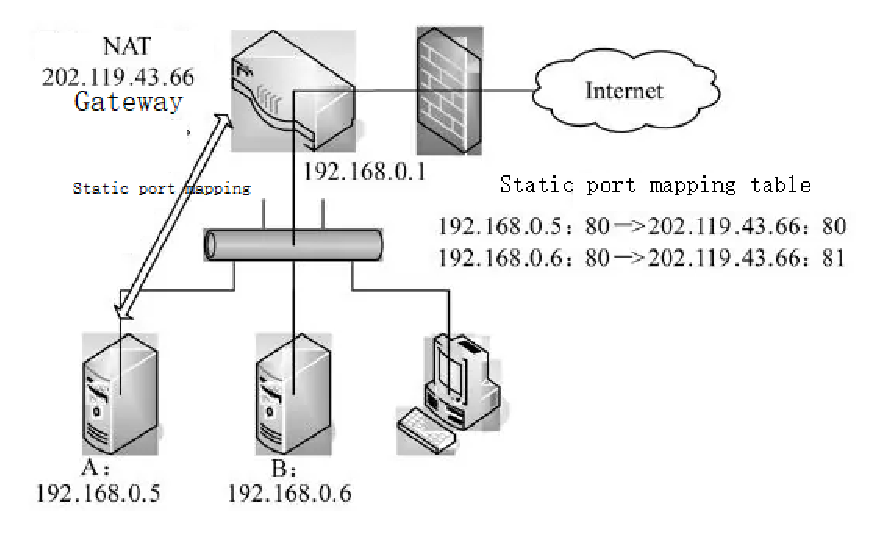
\includegraphics {grafiken/2.14.eps}
	\caption{NAT-Technical} 
	\label{fig:2.14}
\end{figure}
\FloatBarrier
This article uses Ngrok for intranet penetration, the structure is as follows Figure~\ref{fig:2.15} :

% ~\ref{fig:2.15} 
\begin{figure}[!ht]
	\centering
	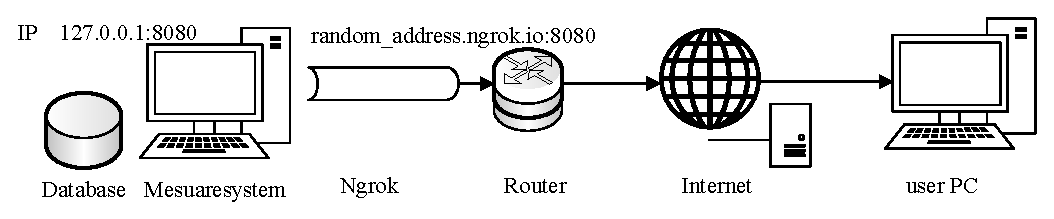
\includegraphics[width=15cm]{grafiken/2.15.eps}
	\caption{Ngrok-Technical realization} 
	\label{fig:2.15}
\end{figure}
\FloatBarrier

\section{IoT}
\label{sec:IoT}
% 2.8
Internet of Things is abbreviated into IoT. 
In brief, it means that all devices are linked to the internet in a way: 
From smartphones and tablet PCs (common) to automobiles and refrigerators 
The main function of IoT lies in how to link devices, services, and Apps to the internet so that it will develop the greater role. There is almost no limitation for devices accessed in the internet and reasons for access. 
The important way for IoT to improve quality of life lies in making data sharing easier. IoT is conducive to streamlining our life. In the long term, it can handle some trifling matters for us. 
This article uses the core philosophy of IoT and issues data collected to the cloud. Users can access the cloud server through HTML5 page to gain the pushed data. If the cloud server breaks down, user PC can collect the PC through VNC remote control. 

The signal collector gains the outer net IP as the server through internal network penetration. The signal collected by the single chip microcomputer through UDP is imported to the database. Users or researchers in other areas can gain the database data of the signal collector through the html webpage (deployed on the free website of githubpage). When the signal collector goes wrong, users can collect the signal machine through VNC remote control. 

The following Figure~\ref{fig:2.16} is a schematic diagram of the Internet of Things structure used in this article:
% ~\ref{fig:2.16} 
\begin{figure}[!ht]
	\centering
	\includegraphics[width=15cm]{grafiken/2.16.pdf}
	\caption{Measuring models using the Internet of Things} 
	\label{fig:2.16}
\end{figure}
\FloatBarrier

The signal acquisition machine obtains the external network IP as a server through the intranet penetration, and collects the signal collected by the single-chip microcomputer through UDP and imports it into the database. Users or researchers in other regions can obtain it through the html web page (which has been deployed on the free website of the github page) Collect the database data of the signal machine. When there is a problem with the signal machine, the user can also remotely control the signal machine through VNC.

 
\chapter{Introduction of measurement circuit}
\label{chap:Introduction of measurement circuit}
% 3.0
This article mainly studies the influence of voltage, current, and temperature on gallium nitride to determine the influence of cosmic rays on gallium nitride. At the same time, the voltage signal and current signal of the measured unit are equivalent. Because of Ohm's law, voltage and current are proportional, so in this measurement process, this article mainly measures the change of voltage and temperature. When cosmic rays affect gallium nitride, the source and drain of gallium nitride are turned on and enter triode mode or saturation mode, that is, gallium nitride cannot work normally because of cosmic rays.

In order to ensure the measurement accuracy, we add an ADC in front of the unit under test. If the gallium nitride is affected by cosmic rays, the ADC measurement value will change from high to low to achieve the measurement purpose. 
\\
\section{Measurement circuit overview}
\label{sec:Measurement circuit overview}
% 3.1
\\
% The following figure shows the basic structure of the measurement system, which is blown using a fuse.
For multiple units under test, we adopt a one-to-one correspondence method, that is, each unit under test corresponds to an ADC for voltage measurement, and IGBT is used as a protection circuit.
The Figure~\ref{fig:3.1} below shows the basic structure of a measurement system for multiple DUTs.
\begin{figure}[!ht]
	\centering
	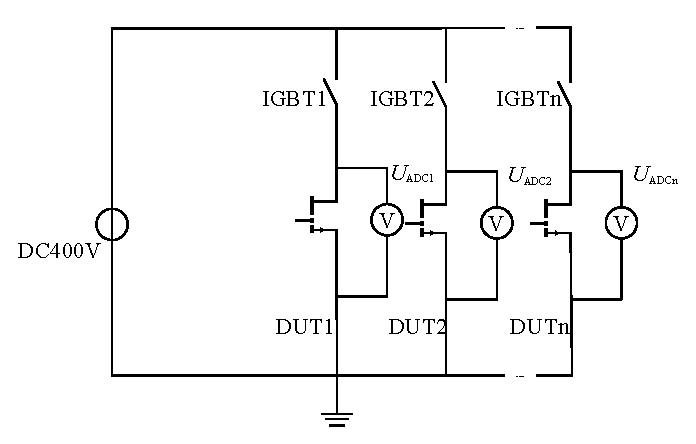
\includegraphics[width=15cm]{grafiken/3.1.eps}
	\caption{Basic structure of the measurement system for multiple DUTs} 
	\label{fig:3.1}
\end{figure}
\FloatBarrier

% When DUT is disturbed by the cosmic rays and it is conductive, the basic circuit uses the fuse as the action circuit. Then, the measuring signal chip suddenly gains a high level and remains the high level. Next, the software system adds one for the error signal counter. The basic constitution of the measuring circuit is shown in Figure  : 
% \\
% In actual use, if we do not consider IGBT control, we can use IGBT as the protecting circuit component. When fusing of the gallium nitride MOSFET is affected by cosmic rays and it is conductive, the microcontroller can gain the voltage value through ADC, so as to realize whether the gallium nitride component will be influenced. The artificial circuit is illustrated below: 
% When DUT is normally operated, IGBT in theory gains a 0V voltage and it will not turn on the microcontroller to get a low level, as shown below: 
% \\
% When DUT is unusually operated, IGBT in theory gets a 15V voltage(with IGBT breakover) and it will not turn on the microcontroller to get a high level, as shown below: 
\\
\section{IGBT control circuit}
\label{sec:IGBT control circuit}
% 3.2
LM393 voltage comparator is used to control IGBT 
LM393 is a common voltage comparator chip in our daily life. It has two independent operational amplifiers. The power supply is provided by wide voltage and undercurrent. Low input controls the current. Generally speaking, the actuation time only has 1.3 microseconds. When the in-phase input voltage is greater than the inverted input voltage, output voltage belongs to the high level. When the in-phase input voltage is less than the inverted input voltage, output voltage belongs to the low level. 

The following figure~\ref{fig:3.1} is a common application circuit of LM393.








The picture above is the artificial circuit of this circuit. The voltage output result is choppy because of LM393’s circuit property. In actual design, the filter capacitor is added to LM393. 

\\
According to STM32F429 official specification, the typical value of STM32 operating power current is 200mAH but we need to select SPI channel and GPIO interface as measurement and use multi-channel ADC for measurement. When the circuit board encounters high temperature and high pressure or improper situations, the required power will rise. Under the circumstance, we need to consider the maximum power (495mW). 
We calculate the main control mainboard’s maximum demanded power by ourselves, thus: 
\\
Since each DCDC chip can provide 6W switching power supply (which provides 350W), each main control mainboard only needs a DCDC convertor). 
We calculate the slave independently, thus: 
\\
In this circuit, the mature SCM chip STM32F429ZG of ST Company is used as the Ethernet-host connection chip. Since STM32F429 has more than 6-line SPI channels, it can be used as the chip to link with various chips. Since each STM32F303ZET6 has more than 40-channel ADC with the high cost performance, STM32F303ZET6 is used as the voltage signal chip for acquisition. 
The specific circuit diagram is shown below: 
\\
To measure 1000 DUT components, at least 1000 lines of ADC should be used. To ensure signal quality, electromagnetic compatibility, and developmental cost, ADC is only used on the slave, as shown in the picture below: 
\\
If we measure 1000 measured units and each STM32F303ZET provides independent 40-line ADC, we need 25 STM32F303 chips. The table below shows the independent ADC distribution of each STM32F303. 
\\

\\
To improve reliability and SNR, this article needs to discuss the upper limit of acquisition speed to ensure that all data will be sent to the PC correctly. 
\\
According to the chip’s specification, SPI of the slave only has the fastest transmission speed of 4Mbps. Moreover, four slave mainboards send data to the host mainboard. Every time, ADC voltage signal acquisition at least needs 1.5 periods and the maximum periods should be set up as 601.5. According to the specification, each switching time is: 
\\
Since we apply the mean filter method, sampling per 10 times can be used as a group of data and then through geometric mean, at least 10us is needed for sampling. 
Considering that the host mainboard accepts the data sent from 5 slave mainboards simultaneously, the SPI receiving speed is set up as 8MB/s, for the sake of preventing congestion. 
Thus, sending speed of each slave mainboard must be reduced to 1.6Mbps, for the sake of ensuring that the host mainboard can receive all data from the slave mainboard. 
In other words, the slave mainboard applies the mean filtering circulation to increase the delay procedure every time, so as to ensure that each value received by the host is valid and reliable. 
At the same time, the temperature collecting speed of the mainboard should be noticed. It will exert an impact on the acquisition speed and total time of major cycles. Developers can set up the counter to set up the number of major cycles to acquire the temperature value once. According to the picture below, 
The host writes data in DS18B20 as writing the time slot, including “0” time slot and “1” time slot. The bus host uses “1” time slot to write logic in DS18B20 and to write logic 0 in DS18B20 as writing “0” time slot. All writing time slots at least must have 60μs duration. Two adjacent writing time slots at least must have 1μs recovery time. Two writing time slots can be generated by lowering the bus through the host (see the picture below), for the sake of generating “1” time slot. 
After lowering the bus, the host must release the bus within 15μs. After releasing the bus, the pull-up resistor can recover the bus to the high level. To generate “0” time slot, after lowering the bus, the host must continue lowering the bus to satisfy the requirement of the time slot’s duration (at least 60μs). 
After the host generates the writing time slots, DS18B20 will sample the single bus(DQ) within a time quantum of 15-60μs. Within the time window of sampling, if the bus belongs to the high level, the host will write 1 in DS18B20; if the bus belongs to the low level, the host will write 0 in DS18B20. 
To sum up, all writing time slots at least must have 60μs of duration. Two adjacent time slots at least must have 1μs of recovery time. All writing time slots(0 and 1) are generated by lowering the bus. 
When the host launches to read the time sequences, DS18B20 is only used to transmit data to the controller, thus the bus controller will issue the order of reading the transient memory [0xBe] or the order of reading the power mode [0xB4] and then it immediately starts reading time sequences. DS18B20 can provide the request information. Besides, the bus controller will read the time sequences after issuing the order of sending temperature conversion[0x44](or recalling EEPROM order[0xB8]) before reading time sequences. See details in the functional order in DS18B20 chip manual. 
All reading time sequences at least must reach 60μs, including two reading periods with at least 1μs recovery time. When the bus controller pulls the USB cable from the high level to the low level, as starting reading time sequences, USB cables at least must remain 1μs and then the bus is released. DS18B20 pulls up or pulls down the bus to transmit “1” or “0”. When the transmission logic “0” comes to an end, the bus will be released. When the pull-up resistor returns to the rising edge state, data from DS18B20 will be valid within 15μs after the falling edge of reading time sequences occurs. Thus, as starting reading time sequences, the bus controller must stop I/O drive into the low voltage 15μs to read I/O state. 
This article produces multi-layer PCB board to ensure signal quality and electromagnetic compatibility. Generally speaking, three kinds of multi-layer board layout modes are illustrated below: 
The designer needs to consider four rules below. 
Also, we need high semaphore of transmission and long-time use. 


\subsection{Simulation of Measurement circuit}
\label{sec:Simulation of Measurement circuit}
% 3.x.x

\section{ }
\label{sec: }
% 3.x

\chapter{Design of the measuring system}
\label{chap:Design of the measuring system}
% 4.x

\chapter{Detailed presentation of the measuring system}
\label{chap:Detailed presentation of the measuring system}
% 5.x


\chapter{Design PCBs}
\label{chap:Design PCBs}
% 6.x

\chapter{Introduce measurement with eval boards }
\label{chap:Introduce measurement with eval boards }
% 7.x
 

\chapter{Conlusion}
\label{chap:Conlusion}
% 8.x
In order to measure the effects of cosmic radiation on GaN power semiconductors for a long time, the microcontroller STM32F303 is used to measure the voltage signal and the DS18b20 is used to measure the temperature signal.
\\
The collected signal is sent to the main control unit of the microprocessor through AD conversion, the data collection stage is realized through database and back-end processing, and the collected data is sent to the front-end to facilitate clearly understanding of the users.
The acquisition circuit is also simulated at the same time, the PCB board is designed and laid out to meet the design requirements.
\\
Researchers can first debug the data which is collected from the host and slave through the debugger, then import the collected data into the MySQL database through the shell command line, and finally convert the IP address of the intranet to the public network address through the intranet penetration. In this case the personnel at the Hannover Institute can also observe changes of the collected signals such as the number of failed units under test. Researchers can also remotely access and control the experimental PC through VNC and collect data from the back-end to the database and then to the front-end. This realized the process of the Internet of Things.

% \chapter{Motordaten}
% \label{app:Motordaten}
\chapter{Appendix}
\label{chap:Appendix}
\\
\section{Slaveboard ADC acquisition part of the program}
\label{sec:Slaveboard ADC acquisition part of the program}
% A.1
\textbf{Arithmetic Average Filter in Slaveboard ADC channel1-channel11}\\
for(i = 0,ad1 =0,ad2=0,ad3=0,ad4=0,ad5 =0,ad6=0,\\ad7=0,ad8=0,ad9 =0,ad10=0,ad11=0; i < 110;)
\\{
\\ad1 += ADC1$_$Value[i++];ad2 += ADC$_$Value[i++];ad3 += ADC$_$Value[i++];
\\ad4 += ADC$_$Value[i++];ad5 += ADC$_$Value[i++];ad6 += ADC$_$Value[i++];
\\ad7 += ADC$_$Value[i++];ad8 += ADC$_$Value[i++];ad9 += ADC$_$Value[i++];
\\ad10 += ADC$_$Value[i++];ad11 += ADC$_$Value[i++];} 
\\ad1 /= 10;ad2 /= 10;ad3 /= 10;
\\ad4 /= 10;ad5 /= 10;ad6 /= 10;
\\ad7 /= 10;ad8 /= 10;ad9 /= 10;
\\ad10 /= 10;ad11 /= 10;
\\
\section{Back end part of the program}
\label{sec:Back end part of the program}
% A.2
\textbf{The back end MybatisPlus automatically generates instances and interfaces of all elements in the database corresponding list}
\\
        dataSourceConfig.setDbType(DbType.MYSQL);        // choose which SQL is used 
      \\
        dataSourceConfig.setDriverName("com.mysql.cj.jdbc.Driver");
       \\
        dataSourceConfig.setUsername("root");
       \\ dataSourceConfig.setPassword("123456"); 
        \\dataSourceConfig.setUrl("jdbc:mysql://localhost:3306/gan");  // choose which Table in MySQL is used 
        \\
        autoGenerator.setDataSource(dataSourceConfig);

      \\  List<TableFill> list = new ArrayList<>();
      \\  TableFill tableFill1 = new TableFill("create$_$time",FieldFill.INSERT);
      \\  TableFill tableFill2 = new TableFill("update$_$time",FieldFill.INSERT$_$UPDATE);
      \\  list$.$add(tableFill1);
      \\  list$.$add(tableFill2);

      \\  strategyConfig.setTableFillList(list);
      \\  autoGenerator.setStrategy(strategyConfig);

      \\  autoGenerator.execute();



% \chapter{Latex: Getting Started}
\label{chap:Latex_Getting_Started}

Zum Arbeiten mit dieser Hilfe bitte  \glqq  Arbeit.tex\grqq{} mit \textit{TexStudio} öffnen und kompilieren (F5). Anschließend kann in der PDF-Ansicht von \textit{TexStudio} per Rechtsklick auf die passende Stelle und \glqq Gehe zu Quelltext\grqq{} der zugehörige Quelltext nachgeschlagen werden. Es handelt sich hierbei nur um Minimalbeispiele um die allerersten Schritte in Latex zu schaffen.

\section{Bilder einfügen}

In Abbildung~\ref{fig:welfenschloss} ist das Welfenschloss dargestellt.
\begin{figure}[h]
	\centering
	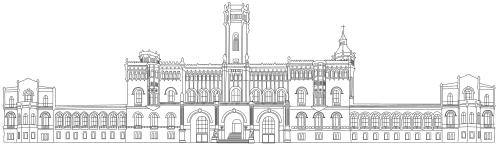
\includegraphics[width=\textwidth]{welfenschloss_vektor}
	\caption{Beispielcaption}
	\label{fig:welfenschloss}
\end{figure} 

\clearpage
\section{Plots}

\subsubsection{Gutes Beispiel}

\begin{figure}[!ht]
	\centering
	\setlength\figureheight{7cm}
	\setlength\figurewidth{13cm}
	% This file was created by matlab2tikz.
%
%The latest updates can be retrieved from
%  http://www.mathworks.com/matlabcentral/fileexchange/22022-matlab2tikz-matlab2tikz
%where you can also make suggestions and rate matlab2tikz.
%
\begin{tikzpicture}

\begin{axis}[%
width=\figurewidth,
height=0.907\figureheight,
at={(0\figurewidth,0\figureheight)},
scale only axis,
separate axis lines,
every outer x axis line/.append style={black},
every x tick label/.append style={font=\color{black}},
xmin=0,
xmax=6,
xtick={0,1,2,3,4,5,6},
xlabel={Zeit in s},
xmajorgrids,
every outer y axis line/.append style={black},
every y tick label/.append style={font=\color{black}},
ymin=-0.6,
ymax=0.6,
ytick={-0.6,-0.4,-0.2,0,0.2,0.4,0.6},
yticklabels={{-0,6},{-0,4},{-0,2},{0},{0,2},{0,4},{0,6}},
ylabel={Strom in A},
ymajorgrids,
axis background/.style={fill=white},
legend style={legend cell align=left,align=left,draw=white!15!black}
]
\addplot [color=black,solid,line width=1.0pt]
  table[row sep=crcr]{%
0	0\\
0.1	0.109268131937284\\
0.2	0.214180088269758\\
0.3	0.31055336036727\\
0.4	0.394545849994738\\
0.5	0.462809041644343\\
0.6	0.512621497281975\\
0.7	0.541997351493653\\
0.8	0.549765481672828\\
0.9	0.535616196983007\\
1	0.500113584754125\\
1.1	0.444673022100775\\
1.2	0.371504749303133\\
1.3	0.283525754501805\\
1.4	0.184243482585748\\
1.5	0.077616004432927\\
1.6	-0.0321057788851691\\
1.7	-0.140547606114757\\
1.8	-0.243386243812169\\
1.9	-0.336521840018496\\
2	-0.416241372419361\\
2.1	-0.479366674827474\\
2.2	-0.523381140639234\\
2.3	-0.546530051998406\\
2.4	-0.547890534859712\\
2.5	-0.527408351064726\\
2.6	-0.485900060646084\\
2.7	-0.425020468155793\\
2.8	-0.347196650829777\\
2.9	-0.255531198677566\\
3	-0.153678524009409\\
3.1	-0.045699171549623\\
3.2	0.0641020626677715\\
3.3	0.171347749932358\\
3.4	0.271762343126234\\
3.5	0.361342629295334\\
3.6	0.436517325117034\\
3.7	0.494289452696395\\
3.8	0.532355819617317\\
3.9	0.549198839956033\\
4	0.54414703564286\\
4.1	0.517401806173875\\
4.2	0.470029399448554\\
4.3	0.403918403830762\\
4.4	0.321704456090469\\
4.5	0.226665166882966\\
4.6	0.122589452755136\\
4.7	0.0136264839993468\\
4.8	-0.0958797296726388\\
4.9	-0.201563521088561\\
5	-0.299211610989153\\
5.1	-0.384931078176448\\
5.2	-0.45530455799711\\
5.3	-0.507526481887044\\
5.4	-0.53951492653657\\
5.5	-0.549994613602887\\
5.6	-0.538547751033225\\
5.7	-0.505630689115572\\
5.8	-0.45255572723279\\
5.9	-0.381438796627417\\
6	-0.295115104900239\\
6.1	-0.197026105230255\\
6.2	-0.0910822964965702\\
};
\addlegendentry{$i_1$};

\addplot [color=blue,dashed,line width=1.0pt]
  table[row sep=crcr]{%
0	0.242487113059643\\
0.1	0.27992203730887\\
0.2	0.248822284202539\\
0.3	0.156802157942887\\
0.4	0.0263913947523759\\
0.5	-0.110480902305586\\
0.6	-0.220303621322969\\
0.7	-0.276188330483089\\
0.8	-0.264452503936179\\
0.9	-0.187969481322183\\
1	-0.0654649740156728\\
1.1	0.0730676421006614\\
1.2	0.193710751107647\\
1.3	0.266926712344854\\
1.4	0.274789705005495\\
1.5	0.21537459425479\\
1.6	0.103228271378942\\
1.7	-0.034191932542297\\
1.8	-0.163240758891846\\
1.9	-0.252322554244172\\
2	-0.279626988260801\\
2.1	-0.238468983219033\\
2.2	-0.138925454188702\\
2.3	-0.00536812877837581\\
2.4	0.129503501776933\\
2.5	0.232668158504726\\
2.6	0.278867535444852\\
2.7	0.25679041386277\\
2.8	0.171842043088305\\
2.9	0.0448207469650515\\
3	-0.0931742311934444\\
3.1	-0.20835690799087\\
3.2	-0.272526547010924\\
3.3	-0.269972182627098\\
3.4	-0.201319212327125\\
3.5	-0.0833762775964814\\
3.6	0.0549800777391185\\
3.7	0.179875392546936\\
3.8	0.260730937885635\\
3.9	0.277750456320574\\
4	0.226766976162424\\
4.1	0.120263031464932\\
4.2	-0.0156854976550285\\
4.3	-0.147793669898183\\
4.4	-0.243716797265827\\
4.5	-0.279969552742338\\
4.6	-0.24767599742802\\
4.7	-0.154742719940931\\
4.8	-0.0239230277712742\\
4.9	0.112753855941553\\
5	0.221824663291686\\
5.1	0.276585056662421\\
5.2	0.263627781921117\\
5.3	0.1861252318252\\
5.4	0.0630527336340797\\
5.5	-0.075457272791626\\
5.6	-0.195492707173551\\
5.7	-0.267664708792873\\
5.8	-0.274303054566629\\
5.9	-0.213782445929001\\
6	-0.100920438604497\\
6.1	0.0366504118137338\\
6.2	0.165247963192162\\
};
\addlegendentry{$i_2$};

\end{axis}
\end{tikzpicture}%
	\caption{Verlauf der Str\"ome auf der Primär- und der Sekundärseite in Abh\"angigkeit von der Zeit} 
	\label{abb:stromverlauf_gutes_bsp}
\end{figure}
\FloatBarrier

\subsubsection{Schlechtes Beispiel}

\begin{figure}[!ht]
	\centering
	\setlength\figureheight{7cm}
	\setlength\figurewidth{14cm}
	% This file was created by matlab2tikz.
%
%The latest updates can be retrieved from
%  http://www.mathworks.com/matlabcentral/fileexchange/22022-matlab2tikz-matlab2tikz
%where you can also make suggestions and rate matlab2tikz.
%
\definecolor{mycolor1}{rgb}{0.00000,1.00000,1.00000}%
%
\begin{tikzpicture}

\begin{axis}[%
width=\figurewidth,
height=0.907\figureheight,
at={(0\figurewidth,0\figureheight)},
scale only axis,
separate axis lines,
every outer x axis line/.append style={black},
every x tick label/.append style={font=\color{black}},
xmin=0,
xmax=7,
xlabel={Zeit in $s$~\Huge\textcolor{red}{7}},
xmajorgrids,
every outer y axis line/.append style={black},
every y tick label/.append style={font=\color{black}},
ymin=-0.5,
ymax=0.5,
ytick={-0.4, -0.2,    0,  0.2,  0.4},
ylabel={Strom [A]~\Huge\textcolor{red}{1}},
ymajorgrids,
axis background/.style={fill=white},
legend style={at={(0.03,0.97)},anchor=north west,legend cell align=left,align=left,draw=white!15!black}
]
\addplot [color=blue,solid,line width=1.0pt]
  table[row sep=crcr]{%
0	0\\
0.1	0.0894011988577775\\
0.2	0.175238254038893\\
0.3	0.254089113027766\\
0.4	0.322810240904785\\
0.5	0.378661943163553\\
0.6	0.419417588685252\\
0.7	0.443452378494807\\
0.8	0.449808121368677\\
0.9	0.438231433895188\\
1	0.409183842071557\\
1.1	0.363823381718816\\
1.2	0.303958431248018\\
1.3	0.231975617319659\\
1.4	0.150744667570157\\
1.5	0.0635040036269403\\
1.6	-0.026268364542411\\
1.7	-0.114993495912074\\
1.8	-0.199134199482684\\
1.9	-0.275336050924224\\
2	-0.340561122888568\\
2.1	-0.392209097586115\\
2.2	-0.428220933250282\\
2.3	-0.447160951635059\\
2.4	-0.448274073976128\\
2.5	-0.431515923598412\\
2.6	-0.397554595074069\\
2.7	-0.347744019400194\\
2.8	-0.284069987042544\\
2.9	-0.20907098073619\\
3	-0.125736974189517\\
3.1	-0.0373902312678734\\
3.2	0.0524471421827221\\
3.3	0.14019361358102\\
3.4	0.222351008012374\\
3.5	0.295643969423455\\
3.6	0.357150538732119\\
3.7	0.404418643115232\\
3.8	0.435563852414169\\
3.9	0.449344505418572\\
4	0.445211210980522\\
4.1	0.423328750505898\\
4.2	0.384569508639726\\
4.3	0.330478694043351\\
4.4	0.263212736801293\\
4.5	0.18545331835879\\
4.6	0.100300461345111\\
4.7	0.011148941454011\\
4.8	-0.0784470515503408\\
4.9	-0.164915608163368\\
5	-0.244809499900216\\
5.1	-0.314943609417094\\
5.2	-0.372521911088544\\
5.3	-0.415248939725763\\
5.4	-0.441421303529921\\
5.5	-0.449995592947817\\
5.6	-0.440629978118093\\
5.7	-0.413697836549104\\
5.8	-0.370272867735919\\
5.9	-0.312086288149705\\
6	-0.241457813100196\\
6.1	-0.161203177006572\\
6.2	-0.0745218789517392\\
};
\addlegendentry{i$_1$};

\addplot [color=mycolor1,solid,line width=1.0pt]
  table[row sep=crcr]{%
0	0.242487113059643\\
0.1	0.27992203730887\\
0.2	0.248822284202539\\
0.3	0.156802157942887\\
0.4	0.0263913947523759\\
0.5	-0.110480902305586\\
0.6	-0.220303621322969\\
0.7	-0.276188330483089\\
0.8	-0.264452503936179\\
0.9	-0.187969481322183\\
1	-0.0654649740156728\\
1.1	0.0730676421006614\\
1.2	0.193710751107647\\
1.3	0.266926712344854\\
1.4	0.274789705005495\\
1.5	0.21537459425479\\
1.6	0.103228271378942\\
1.7	-0.034191932542297\\
1.8	-0.163240758891846\\
1.9	-0.252322554244172\\
2	-0.279626988260801\\
2.1	-0.238468983219033\\
2.2	-0.138925454188702\\
2.3	-0.00536812877837581\\
2.4	0.129503501776933\\
2.5	0.232668158504726\\
2.6	0.278867535444852\\
2.7	0.25679041386277\\
2.8	0.171842043088305\\
2.9	0.0448207469650515\\
3	-0.0931742311934444\\
3.1	-0.20835690799087\\
3.2	-0.272526547010924\\
3.3	-0.269972182627098\\
3.4	-0.201319212327125\\
3.5	-0.0833762775964814\\
3.6	0.0549800777391185\\
3.7	0.179875392546936\\
3.8	0.260730937885635\\
3.9	0.277750456320574\\
4	0.226766976162424\\
4.1	0.120263031464932\\
4.2	-0.0156854976550285\\
4.3	-0.147793669898183\\
4.4	-0.243716797265827\\
4.5	-0.279969552742338\\
4.6	-0.24767599742802\\
4.7	-0.154742719940931\\
4.8	-0.0239230277712742\\
4.9	0.112753855941553\\
5	0.221824663291686\\
5.1	0.276585056662421\\
5.2	0.263627781921117\\
5.3	0.1861252318252\\
5.4	0.0630527336340797\\
5.5	-0.075457272791626\\
5.6	-0.195492707173551\\
5.7	-0.267664708792873\\
5.8	-0.274303054566629\\
5.9	-0.213782445929001\\
6	-0.100920438604497\\
6.1	0.0366504118137338\\
6.2	0.165247963192162\\
};
\addlegendentry{$i_2$};
\node[font=\bfseries] at (0.2,-0.42) {\Huge\textcolor{red}{2}};
\node[font=\bfseries] at (1,0.45) {\Huge\textcolor{red}{3}};
\node[font=\bfseries] at (1,0.34) {\Huge\textcolor{red}{4}};
\node[font=\bfseries] at (6.5,0.4) {\Huge\textcolor{red}{5}};
\node[font=\bfseries] at (6.5,0) {\Huge\textcolor{red}{6}};
\node[font=\bfseries] at (2.2,0.07) {\Huge\textcolor{red}{9}};
\end{axis}
\end{tikzpicture}%
	\caption{Str\"ome in Abh\"angigkeit der Zeit~\Huge\textcolor{red}{8}} 
	\label{abb:stromverlauf_schlechtes_bsp}
\end{figure}
\FloatBarrier
\newpage


\subsubsection{Erläuterungen zum Plot}

\begin{enumerate}
	\item[1)] Einheiten nicht in eckige Klammer schreiben. Richtig ist:
	\begin{itemize}
		\item Strom in A
		\item Strom /A
		\item Strom $i$ in A
		\item Strom $i$ /A
		\item $i$ in A
		\item $i$ /A
		\item Wichtig ist: immer eine einheitliche Darstellung verwenden
		\item zur Info: diese Schreibweise ist korrekt: [$i$]~=~A, wird aber nicht als Achsenbeschriftung verwendet
	\end{itemize}
	\item[2)] In deutschen Arbeiten Dezimalkomma verwenden. In englischen Veröffentlichungen Dezimalpunkte verwenden.
	\item[3)] Indizes gerade (es sei denn, der Index ist eine Variable, z.B. Zählvariable)
	\item[4)] Legende muss an einer günstigen Stelle platziert sein, möglichst Verdeckung vermeiden
	\item[5)] Abbildung darf nicht über den Rand des Dokuments ragen
	\item[6)] Verläufe sollten bis zum Ende des Plots gehen. Die Achse muss nicht zwingend mit einem Zahlenwert abgeschlossen werden.
	\item[7)] Einheiten immer gerade schreiben, nicht kursiv
	\item[8)] Es heißt immer: in Abhängigkeit \textbf{von} ...
	\item[9)] Geeignete Plotfarben wählen, die gut erkennbar sind. Für s/w-Ausdrucke ist es sinnvoll auch die Art des Plots zu unterscheiden (durchgezogen, gestrichelt, gepunktet, markiert)
\end{enumerate}

\subsubsection{Tipps}

\begin{itemize}
	\item Bildunterschrift muss vollständig und eindeutig sein
	\item Möglichst nicht mehr als drei bis vier Verläufe pro Plot abbilden
	\item Skalierung der Achsen sinnvoll wählen
\end{itemize}

\section{Tabellen}

Tabellen sind recht umfangreich und etwas aufwendiger als in Word. Gute Beispiele gibt es unter anderem hier: \href{https://en.wikibooks.org/wiki/LaTeX/Tables}{https://en.wikibooks.org/wiki/LaTeX/Tables}.

\section{Gleichungen}

\subsection{Einheiten}
Einheiten sind nicht kursiv zu schreiben. Da dies innerhalb der Mathematikumgebung häufig schief geht, wird empfohlen den Befehl \verb=$\SI{40}{\N\m}$= zu verwenden. Die Darstellung von Einheiten kann dadurch global eingestellt werden (immer gerade, Einheiten mit Bruchstrich oder negativen Exponenten, Komma als Dezimaltrenner, usw.).

Beispiel:

Damit beträgt das Drehmoment beträgt $M=\SI{40}{\N\m}$.

Weitere Beispiele:
\begin{enumerate}
	\item $\SI{1}{\meter\per\square\second}$
	\item $\SI{100}{\nano\farad}$
	\item $\SI{100}{\mega\var}$
\end{enumerate}
Neue Einheiten können über  \verb!\DeclareSIUnit \var {var}! in \glqq  Pakete.tex\grqq{} erstellt werden.

\section{Literaturverweise setzen}

In \cite{ASYN:2001} sind die notwendigen Formeln dargestellt.
\include{Auswertung}


%%%%%%%%%%%%%%%%%%%%%%%%%%%%%%%%%%%%%%%%%%%%%%%%%%%%%%%%%%%%%%%%%%%%%%%%%%%%%%%%%%%%%%%%%
%Anhang
\clearpage{\thispagestyle{empty}\cleardoublepage}				% Anhang auf rechter Seite beginnen
\begin{appendix}
% \chapter{Motordaten}
% \label{app:Motordaten}
\chapter{Appendix}
\label{chap:Appendix}
\\
\section{Slaveboard ADC acquisition part of the program}
\label{sec:Slaveboard ADC acquisition part of the program}
% A.1
\textbf{Arithmetic Average Filter in Slaveboard ADC channel1-channel11}\\
for(i = 0,ad1 =0,ad2=0,ad3=0,ad4=0,ad5 =0,ad6=0,\\ad7=0,ad8=0,ad9 =0,ad10=0,ad11=0; i < 110;)
\\{
\\ad1 += ADC1$_$Value[i++];ad2 += ADC$_$Value[i++];ad3 += ADC$_$Value[i++];
\\ad4 += ADC$_$Value[i++];ad5 += ADC$_$Value[i++];ad6 += ADC$_$Value[i++];
\\ad7 += ADC$_$Value[i++];ad8 += ADC$_$Value[i++];ad9 += ADC$_$Value[i++];
\\ad10 += ADC$_$Value[i++];ad11 += ADC$_$Value[i++];} 
\\ad1 /= 10;ad2 /= 10;ad3 /= 10;
\\ad4 /= 10;ad5 /= 10;ad6 /= 10;
\\ad7 /= 10;ad8 /= 10;ad9 /= 10;
\\ad10 /= 10;ad11 /= 10;
\\
\section{Back end part of the program}
\label{sec:Back end part of the program}
% A.2
\textbf{The back end MybatisPlus automatically generates instances and interfaces of all elements in the database corresponding list}
\\
        dataSourceConfig.setDbType(DbType.MYSQL);        // choose which SQL is used 
      \\
        dataSourceConfig.setDriverName("com.mysql.cj.jdbc.Driver");
       \\
        dataSourceConfig.setUsername("root");
       \\ dataSourceConfig.setPassword("123456"); 
        \\dataSourceConfig.setUrl("jdbc:mysql://localhost:3306/gan");  // choose which Table in MySQL is used 
        \\
        autoGenerator.setDataSource(dataSourceConfig);

      \\  List<TableFill> list = new ArrayList<>();
      \\  TableFill tableFill1 = new TableFill("create$_$time",FieldFill.INSERT);
      \\  TableFill tableFill2 = new TableFill("update$_$time",FieldFill.INSERT$_$UPDATE);
      \\  list$.$add(tableFill1);
      \\  list$.$add(tableFill2);

      \\  strategyConfig.setTableFillList(list);
      \\  autoGenerator.setStrategy(strategyConfig);

      \\  autoGenerator.execute();



\end{appendix}


% % \chapter{Motordaten}
% \label{app:Motordaten}
\chapter{Appendix}
\label{chap:Appendix}
\\
\section{Slaveboard ADC acquisition part of the program}
\label{sec:Slaveboard ADC acquisition part of the program}
% A.1
\textbf{Arithmetic Average Filter in Slaveboard ADC channel1-channel11}\\
for(i = 0,ad1 =0,ad2=0,ad3=0,ad4=0,ad5 =0,ad6=0,\\ad7=0,ad8=0,ad9 =0,ad10=0,ad11=0; i < 110;)
\\{
\\ad1 += ADC1$_$Value[i++];ad2 += ADC$_$Value[i++];ad3 += ADC$_$Value[i++];
\\ad4 += ADC$_$Value[i++];ad5 += ADC$_$Value[i++];ad6 += ADC$_$Value[i++];
\\ad7 += ADC$_$Value[i++];ad8 += ADC$_$Value[i++];ad9 += ADC$_$Value[i++];
\\ad10 += ADC$_$Value[i++];ad11 += ADC$_$Value[i++];} 
\\ad1 /= 10;ad2 /= 10;ad3 /= 10;
\\ad4 /= 10;ad5 /= 10;ad6 /= 10;
\\ad7 /= 10;ad8 /= 10;ad9 /= 10;
\\ad10 /= 10;ad11 /= 10;
\\
\section{Back end part of the program}
\label{sec:Back end part of the program}
% A.2
\textbf{The back end MybatisPlus automatically generates instances and interfaces of all elements in the database corresponding list}
\\
        dataSourceConfig.setDbType(DbType.MYSQL);        // choose which SQL is used 
      \\
        dataSourceConfig.setDriverName("com.mysql.cj.jdbc.Driver");
       \\
        dataSourceConfig.setUsername("root");
       \\ dataSourceConfig.setPassword("123456"); 
        \\dataSourceConfig.setUrl("jdbc:mysql://localhost:3306/gan");  // choose which Table in MySQL is used 
        \\
        autoGenerator.setDataSource(dataSourceConfig);

      \\  List<TableFill> list = new ArrayList<>();
      \\  TableFill tableFill1 = new TableFill("create$_$time",FieldFill.INSERT);
      \\  TableFill tableFill2 = new TableFill("update$_$time",FieldFill.INSERT$_$UPDATE);
      \\  list$.$add(tableFill1);
      \\  list$.$add(tableFill2);

      \\  strategyConfig.setTableFillList(list);
      \\  autoGenerator.setStrategy(strategyConfig);

      \\  autoGenerator.execute();



%%%%%%%%%%%%%%%%%%%%%%%%%%%%%%%%%%%%%%%%%%%%%%%%%%%%%%%%%%%%%%%%%%%%%%%%%%%%%%%%%%%%%%%%%
%Literaturverzeichnis

% \bibliography{Literaturverzeichnis}
% \clearpage

%%%%%%%%%%%%%%%%%%%%%%%%%%%%%%%%%%%%%%%%%%%%%%%%%%%%%%%%%%%%%%%%%%%%%%%%%%%%%%%%%%%%%%%%%
%Ende des Dokuments
\end{document} 